\documentclass[twoside]{book}

% Packages required by doxygen
\usepackage{calc}
\usepackage{doxygen}
\usepackage{graphicx}
\usepackage[utf8]{inputenc}
\usepackage{makeidx}
\usepackage{multicol}
\usepackage{multirow}
\usepackage{textcomp}
\usepackage[table]{xcolor}

% Font selection
\usepackage[T1]{fontenc}
\usepackage{mathptmx}
\usepackage[scaled=.90]{helvet}
\usepackage{courier}
\usepackage{amssymb}
\usepackage{sectsty}
\renewcommand{\familydefault}{\sfdefault}
\allsectionsfont{%
  \fontseries{bc}\selectfont%
  \color{darkgray}%
}
\renewcommand{\DoxyLabelFont}{%
  \fontseries{bc}\selectfont%
  \color{darkgray}%
}

% Page & text layout
\usepackage{geometry}
\geometry{%
  a4paper,%
  top=2.5cm,%
  bottom=2.5cm,%
  left=2.5cm,%
  right=2.5cm%
}
\tolerance=750
\hfuzz=15pt
\hbadness=750
\setlength{\emergencystretch}{15pt}
\setlength{\parindent}{0cm}
\setlength{\parskip}{0.2cm}
\makeatletter
\renewcommand{\paragraph}{%
  \@startsection{paragraph}{4}{0ex}{-1.0ex}{1.0ex}{%
    \normalfont\normalsize\bfseries\SS@parafont%
  }%
}
\renewcommand{\subparagraph}{%
  \@startsection{subparagraph}{5}{0ex}{-1.0ex}{1.0ex}{%
    \normalfont\normalsize\bfseries\SS@subparafont%
  }%
}
\makeatother

% Headers & footers
\usepackage{fancyhdr}
\pagestyle{fancyplain}
\fancyhead[LE]{\fancyplain{}{\bfseries\thepage}}
\fancyhead[CE]{\fancyplain{}{}}
\fancyhead[RE]{\fancyplain{}{\bfseries\leftmark}}
\fancyhead[LO]{\fancyplain{}{\bfseries\rightmark}}
\fancyhead[CO]{\fancyplain{}{}}
\fancyhead[RO]{\fancyplain{}{\bfseries\thepage}}
\fancyfoot[LE]{\fancyplain{}{}}
\fancyfoot[CE]{\fancyplain{}{}}
\fancyfoot[RE]{\fancyplain{}{\bfseries\scriptsize Generated on Mon Feb 25 2019 17\-:01\-:26 for Molssi Driver Interface Library by Doxygen }}
\fancyfoot[LO]{\fancyplain{}{\bfseries\scriptsize Generated on Mon Feb 25 2019 17\-:01\-:26 for Molssi Driver Interface Library by Doxygen }}
\fancyfoot[CO]{\fancyplain{}{}}
\fancyfoot[RO]{\fancyplain{}{}}
\renewcommand{\footrulewidth}{0.4pt}
\renewcommand{\chaptermark}[1]{%
  \markboth{#1}{}%
}
\renewcommand{\sectionmark}[1]{%
  \markright{\thesection\ #1}%
}

% Indices & bibliography
\usepackage{natbib}
\usepackage[titles]{tocloft}
\setcounter{tocdepth}{3}
\setcounter{secnumdepth}{5}
\makeindex

% Hyperlinks (required, but should be loaded last)
\usepackage{ifpdf}
\ifpdf
  \usepackage[pdftex,pagebackref=true]{hyperref}
\else
  \usepackage[ps2pdf,pagebackref=true]{hyperref}
\fi
\hypersetup{%
  colorlinks=true,%
  linkcolor=blue,%
  citecolor=blue,%
  unicode%
}

% Custom commands
\newcommand{\clearemptydoublepage}{%
  \newpage{\pagestyle{empty}\cleardoublepage}%
}


%===== C O N T E N T S =====

\begin{document}

% Titlepage & ToC
\hypersetup{pageanchor=false}
\pagenumbering{roman}
\begin{titlepage}
\vspace*{7cm}
\begin{center}%
{\Large Molssi Driver Interface Library }\\
\vspace*{1cm}
{\large Generated by Doxygen 1.8.5}\\
\vspace*{0.5cm}
{\small Mon Feb 25 2019 17:01:26}\\
\end{center}
\end{titlepage}
\clearemptydoublepage
\tableofcontents
\clearemptydoublepage
\pagenumbering{arabic}
\hypersetup{pageanchor=true}

%--- Begin generated contents ---
\chapter{Main Page}
\label{index}\hypertarget{index}{}\hypertarget{index_mainpage_overview_sec}{}\doxysection{Overview}\label{index_mainpage_overview_sec}
The Mol\+S\+SI Driver Interface (M\+DI) seeks to simplify the process of interoperating computational molecular sciences codes. M\+DI uses a driver/engine paradigm in which \mbox{\hyperlink{index_main_doc_drivers_sec}{drivers}} orchestrate complex simulations by controlling \mbox{\hyperlink{index_main_doc_engines_sec}{engines}} through the use of an A\+P\+I-\/like command set that is defined by the \mbox{\hyperlink{mdi_standard}{M\+DI Standard}}. The process of communicating commands and other data between codes is handled by the \mbox{\hyperlink{index_mainpage_overview_sec}{M\+DI Library}}.

In total, M\+DI consists of the following components\+:


\begin{DoxyItemize}
\item \mbox{\hyperlink{index_main_doc_drivers_sec}{Drivers}}, which are codes that control the high-\/level program flow of one or more other codes.
\item \mbox{\hyperlink{index_main_doc_engines_sec}{Engines}}, which are codes capable of responding to commands from an external driver.
\item \mbox{\hyperlink{mdi_standard}{The M\+DI Standard}}, which is an A\+P\+I-\/like definition of a set of commands that can be sent from a driver to an engine, and that cause the engine to respond in a clearly defined way.
\item \mbox{\hyperlink{library_page}{The M\+DI Library}}, which is a library that enables inter-\/code communication in compliance with the M\+DI Standard.
\end{DoxyItemize}\hypertarget{index_mainpage_capabilities_sec}{}\doxysection{Capabilities}\label{index_mainpage_capabilities_sec}
M\+DI is designed to support a wide variety of different calculation types, with the \mbox{\hyperlink{mdi_standard}{M\+DI Standard}} defining a variety of simple commands that can be used to develop many drivers for many purposes. Potential application areas for M\+DI include {\itshape  ab initio} molecular dynamics (A\+I\+MD), path integral molecular dynamics (P\+I\+MD), advanced sampling, forcefield development, and Q\+M/\+MM. More specifically, here are some examples of what can be accomplished using M\+DI\+:


\begin{DoxyItemize}
\item Run an {\itshape  ab initio} molecular dynamics (A\+I\+MD) calculation in which a quantum mechanics (QM) code calculates nuclear forces and a molecular mechancis (MM) code performs the time integration.
\item Run an MD simulation in which the nuclear forces include contributions from two different MM codes.
\item Implement an advanced sampling technique ({\itshape i.\+e.} metadynamics, replica exchange, etc.) in a self-\/contained driver that can use other codes to compute forces.
\item Implement a new forcefield in a self-\/contained engine that is compatible with multiple MM codes.
\item Run Q\+M/\+MM simulations.
\end{DoxyItemize}

Creation of unofficial extensions to the M\+DI Standard is straightforward. Feel free to contact us if your use case requires additions to the M\+DI Standard, and we may be able to provide advice about the process. Extensions that prove useful to the broader community may be considered for official incorporation into the M\+DI Standard.\hypertarget{index_mainpage_getting_started_sec}{}\doxysection{Getting Started}\label{index_mainpage_getting_started_sec}
For guidance on running simulations using M\+D\+I-\/based drivers and engines, please first complete the \mbox{\hyperlink{tutorials_user_tutorial}{User Tutorial}}. Afterwards, please read \mbox{\hyperlink{library_page_library_launching_sec}{Launching Codes with the M\+DI Library}}.

If you intend to develop an M\+D\+I-\/based driver or engine, first do the above. Then, complete the \mbox{\hyperlink{tutorials_aimd_tutorial}{Driver Development Tutorial}} and familiarize yourself with the \mbox{\hyperlink{library_page_functions_sec}{M\+DI Library Functions}}.

For lists of available M\+D\+I-\/based drivers and engines, see \mbox{\hyperlink{index_main_doc_drivers_sec}{Drivers}} and \mbox{\hyperlink{index_main_doc_engines_sec}{Engines}}.\hypertarget{index_source_sec}{}\doxysection{Source Code}\label{index_source_sec}
The source code of the M\+DI library is available at Git\+Hub at \href{https://github.com/MolSSI/MDI_Library}{\texttt{ https\+://github.\+com/\+Mol\+S\+S\+I/\+M\+D\+I\+\_\+\+Library}}\hypertarget{index_main_doc_sec}{}\doxysection{Main Documentation}\label{index_main_doc_sec}

\begin{DoxyItemize}
\item \mbox{\hyperlink{tutorials}{Tutorials}}
\begin{DoxyItemize}
\item \mbox{\hyperlink{tutorials_user_tutorial}{User Tutorial}}
\item \mbox{\hyperlink{tutorials_aimd_tutorial}{Driver Development Tutorial}}
\end{DoxyItemize}
\item \mbox{\hyperlink{mdi_standard}{M\+DI Standard}}
\item \mbox{\hyperlink{library_page}{M\+DI Library}}
\end{DoxyItemize}\hypertarget{index_main_doc_engines_sec}{}\doxysection{Engines}\label{index_main_doc_engines_sec}
The following codes support M\+DI\+:


\begin{DoxyItemize}
\item \href{https://github.com/MolSSI/lammps/tree/mdi}{\texttt{ L\+A\+M\+M\+PS}}
\item \href{https://github.com/MolSSI/q-e/tree/mdi}{\texttt{ Quantum E\+S\+P\+R\+E\+S\+SO}}
\end{DoxyItemize}

The following codes support \href{http://ipi-code.org/}{\texttt{ i-\/\+PI}}, with which M\+DI is compatible (see the \mbox{\hyperlink{library_page_library_launching_sec}{-\/ipi}} option). Note that the i-\/\+PI command set is different from that of the M\+DI Standard.


\begin{DoxyItemize}
\item \href{https://www.cp2k.org/}{\texttt{ C\+P2K}}
\item \href{http://www.dftbplus.org/}{\texttt{ D\+F\+T\+B+}}
\item \href{https://departments.icmab.es/leem/siesta/}{\texttt{ Siesta}}
\item \href{https://aimsclub.fhi-berlin.mpg.de/}{\texttt{ F\+H\+I-\/aims}}
\item \href{http://molmod.github.io/yaff/}{\texttt{ Yaff}}
\item \href{http://demon-nano.ups-tlse.fr/}{\texttt{ de\+Mon\+Nano}}
\item \href{https://www.questaal.org/}{\texttt{ T\+BE}}
\end{DoxyItemize}\hypertarget{index_main_doc_drivers_sec}{}\doxysection{Drivers}\label{index_main_doc_drivers_sec}

\begin{DoxyItemize}
\item \href{https://github.com/MolSSI/MDI_AIMD_Driver}{\texttt{ M\+DI A\+I\+MD Driver}}
\end{DoxyItemize}\hypertarget{index_main_doc_bugs_sec}{}\doxysection{Reporting Bugs, Issues, and Improvements}\label{index_main_doc_bugs_sec}
Bugs and suggestions for improvements can be reported via \href{https://github.com/MolSSI/MDI_Library/issues}{\texttt{ Git\+Hub Issues}} or by emailing the main author directly.\hypertarget{index_main_doc_author_sec}{}\doxysection{Authors}\label{index_main_doc_author_sec}
The M\+DI Library is primarily written by Taylor Barnes $<$\href{mailto:tbarnes1@vt.edu}{\texttt{ tbarnes1@vt.\+edu}}$>$, a Software Scientist at Mol\+S\+SI.\hypertarget{index_main_doc_license_sec}{}\doxysection{License}\label{index_main_doc_license_sec}
The M\+DI Library is released under the 3-\/Clause B\+SD License. See the L\+I\+C\+E\+N\+SE file for more details.\hypertarget{index_main_doc_ack_sec}{}\doxysection{Acknowledgements}\label{index_main_doc_ack_sec}
This work was supported by the Molecular Sciences Software Institute under U.\+S. National Science Foundation grant A\+C\+I-\/1547580. 
\chapter{Namespace Index}
\section{Namespace List}
Here is a list of all documented namespaces with brief descriptions\-:\begin{DoxyCompactList}
\item\contentsline{section}{\hyperlink{namespacemolssi__driver__interface_1_1mdi__python}{molssi\-\_\-driver\-\_\-interface.\-mdi\-\_\-python} }{\pageref{namespacemolssi__driver__interface_1_1mdi__python}}{}
\end{DoxyCompactList}

\chapter{Hierarchical Index}
\section{Class Hierarchy}
This inheritance list is sorted roughly, but not completely, alphabetically\-:\begin{DoxyCompactList}
\item \contentsline{section}{Communicator}{\pageref{classCommunicator}}{}
\begin{DoxyCompactList}
\item \contentsline{section}{Communicator\-M\-P\-I}{\pageref{classCommunicatorMPI}}{}
\item \contentsline{section}{Communicator\-T\-C\-P}{\pageref{classCommunicatorTCP}}{}
\end{DoxyCompactList}
\item \contentsline{section}{mdi}{\pageref{classmdi}}{}
\item \contentsline{section}{mdi\-:\-:M\-D\-I\-\_\-\-Accept\-\_\-\-Communicator\-\_\-}{\pageref{interfacemdi_1_1MDI__Accept__Communicator__}}{}
\item \contentsline{section}{mdi\-:\-:M\-D\-I\-\_\-\-Conversion\-\_\-\-Factor\-\_\-}{\pageref{interfacemdi_1_1MDI__Conversion__Factor__}}{}
\item \contentsline{section}{mdi\-:\-:M\-D\-I\-\_\-\-Init\-\_\-}{\pageref{interfacemdi_1_1MDI__Init__}}{}
\item \contentsline{section}{mdi\-:\-:mdi\-\_\-recv}{\pageref{interfacemdi_1_1mdi__recv}}{}
\item \contentsline{section}{mdi\-:\-:M\-D\-I\-\_\-\-Recv\-\_\-}{\pageref{interfacemdi_1_1MDI__Recv__}}{}
\item \contentsline{section}{mdi\-:\-:M\-D\-I\-\_\-\-Recv\-\_\-\-Command\-\_\-}{\pageref{interfacemdi_1_1MDI__Recv__Command__}}{}
\item \contentsline{section}{mdi\-:\-:mdi\-\_\-send}{\pageref{interfacemdi_1_1mdi__send}}{}
\item \contentsline{section}{mdi\-:\-:M\-D\-I\-\_\-\-Send\-\_\-}{\pageref{interfacemdi_1_1MDI__Send__}}{}
\item \contentsline{section}{mdi\-:\-:M\-D\-I\-\_\-\-Send\-\_\-\-Command\-\_\-}{\pageref{interfacemdi_1_1MDI__Send__Command__}}{}
\end{DoxyCompactList}

\chapter{Class Index}
\section{Class List}
Here are the classes, structs, unions and interfaces with brief descriptions\-:\begin{DoxyCompactList}
\item\contentsline{section}{\hyperlink{structcommunicator__struct}{communicator\-\_\-struct} }{\pageref{structcommunicator__struct}}{}
\item\contentsline{section}{\hyperlink{structdynamic__array__struct}{dynamic\-\_\-array\-\_\-struct} }{\pageref{structdynamic__array__struct}}{}
\item\contentsline{section}{\hyperlink{classmdi}{mdi} }{\pageref{classmdi}}{}
\item\contentsline{section}{\hyperlink{interfacemdi_1_1MDI__Accept__Connection__}{mdi\-::\-M\-D\-I\-\_\-\-Accept\-\_\-\-Connection\-\_\-} }{\pageref{interfacemdi_1_1MDI__Accept__Connection__}}{}
\item\contentsline{section}{\hyperlink{interfacemdi_1_1MDI__Listen__}{mdi\-::\-M\-D\-I\-\_\-\-Listen\-\_\-} }{\pageref{interfacemdi_1_1MDI__Listen__}}{}
\item\contentsline{section}{\hyperlink{interfacemdi_1_1MDI__MPI__Comm__}{mdi\-::\-M\-D\-I\-\_\-\-M\-P\-I\-\_\-\-Comm\-\_\-} }{\pageref{interfacemdi_1_1MDI__MPI__Comm__}}{}
\item\contentsline{section}{\hyperlink{interfacemdi_1_1mdi__recv}{mdi\-::mdi\-\_\-recv} }{\pageref{interfacemdi_1_1mdi__recv}}{}
\item\contentsline{section}{\hyperlink{interfacemdi_1_1MDI__Recv__}{mdi\-::\-M\-D\-I\-\_\-\-Recv\-\_\-} }{\pageref{interfacemdi_1_1MDI__Recv__}}{}
\item\contentsline{section}{\hyperlink{interfacemdi_1_1MDI__Recv__Command__}{mdi\-::\-M\-D\-I\-\_\-\-Recv\-\_\-\-Command\-\_\-} }{\pageref{interfacemdi_1_1MDI__Recv__Command__}}{}
\item\contentsline{section}{\hyperlink{interfacemdi_1_1MDI__Request__Connection__}{mdi\-::\-M\-D\-I\-\_\-\-Request\-\_\-\-Connection\-\_\-} }{\pageref{interfacemdi_1_1MDI__Request__Connection__}}{}
\item\contentsline{section}{\hyperlink{interfacemdi_1_1mdi__send}{mdi\-::mdi\-\_\-send} }{\pageref{interfacemdi_1_1mdi__send}}{}
\item\contentsline{section}{\hyperlink{interfacemdi_1_1MDI__Send__}{mdi\-::\-M\-D\-I\-\_\-\-Send\-\_\-} }{\pageref{interfacemdi_1_1MDI__Send__}}{}
\item\contentsline{section}{\hyperlink{interfacemdi_1_1MDI__Send__Command__}{mdi\-::\-M\-D\-I\-\_\-\-Send\-\_\-\-Command\-\_\-} }{\pageref{interfacemdi_1_1MDI__Send__Command__}}{}
\end{DoxyCompactList}

\chapter{File Index}
\section{File List}
Here is a list of all documented files with brief descriptions\-:\begin{DoxyCompactList}
\item\contentsline{section}{/home/tbarnes/mdi/molssi\-\_\-driver\-\_\-interface/molssi\-\_\-driver\-\_\-interface/\hyperlink{communicator_8cpp}{communicator.\-cpp} \\*Class definition for handling communication between connect codes }{\pageref{communicator_8cpp}}{}
\item\contentsline{section}{/home/tbarnes/mdi/molssi\-\_\-driver\-\_\-interface/molssi\-\_\-driver\-\_\-interface/\hyperlink{communicator_8h}{communicator.\-h} \\*Class declaration for handling communication between connected codes }{\pageref{communicator_8h}}{}
\item\contentsline{section}{/home/tbarnes/mdi/molssi\-\_\-driver\-\_\-interface/molssi\-\_\-driver\-\_\-interface/\hyperlink{mdi_8cpp}{mdi.\-cpp} \\*Functions callable by users of the Mol\-S\-S\-I Driver Interface }{\pageref{mdi_8cpp}}{}
\item\contentsline{section}{/home/tbarnes/mdi/molssi\-\_\-driver\-\_\-interface/molssi\-\_\-driver\-\_\-interface/{\bfseries mdi.\-h} }{\pageref{mdi_8h}}{}
\item\contentsline{section}{/home/tbarnes/mdi/molssi\-\_\-driver\-\_\-interface/molssi\-\_\-driver\-\_\-interface/\hyperlink{mdi__global_8cpp}{mdi\-\_\-global.\-cpp} \\*Global parameters used by the Mol\-S\-S\-I Driver Interface }{\pageref{mdi__global_8cpp}}{}
\item\contentsline{section}{/home/tbarnes/mdi/molssi\-\_\-driver\-\_\-interface/molssi\-\_\-driver\-\_\-interface/{\bfseries mdi\-\_\-global.\-h} }{\pageref{mdi__global_8h}}{}
\end{DoxyCompactList}

\chapter{Namespace Documentation}
\hypertarget{namespacemolssi__driver__interface_1_1mdi}{}\doxysection{molssi\+\_\+driver\+\_\+interface.\+mdi Namespace Reference}
\label{namespacemolssi__driver__interface_1_1mdi}\index{molssi\_driver\_interface.mdi@{molssi\_driver\_interface.mdi}}
\doxysubsection*{Functions}
\begin{DoxyCompactItemize}
\item 
\mbox{\Hypertarget{namespacemolssi__driver__interface_1_1mdi_ac42ca419a43f807072d15c2acb2c130c}\label{namespacemolssi__driver__interface_1_1mdi_ac42ca419a43f807072d15c2acb2c130c}} 
def {\bfseries M\+D\+I\+\_\+\+Init} (arg1, comm)
\item 
\mbox{\Hypertarget{namespacemolssi__driver__interface_1_1mdi_ae2a68f93ef9beb192bb354f651fce4af}\label{namespacemolssi__driver__interface_1_1mdi_ae2a68f93ef9beb192bb354f651fce4af}} 
def {\bfseries M\+D\+I\+\_\+\+Get\+\_\+\+Intra\+\_\+\+Code\+\_\+\+M\+P\+I\+\_\+\+Comm} ()
\item 
def \mbox{\hyperlink{namespacemolssi__driver__interface_1_1mdi_ab81f0bee8f7e5264402a96b8009a7cc6}{M\+D\+I\+\_\+\+Accept\+\_\+\+Communicator}} ()
\begin{DoxyCompactList}\small\item\em Accept a new M\+DI communicator. \end{DoxyCompactList}\item 
\mbox{\Hypertarget{namespacemolssi__driver__interface_1_1mdi_acf395e15d31948c07c8137ed0b50d25c}\label{namespacemolssi__driver__interface_1_1mdi_acf395e15d31948c07c8137ed0b50d25c}} 
def {\bfseries M\+D\+I\+\_\+\+Send} (arg1, arg2, arg3, arg4)
\item 
\mbox{\Hypertarget{namespacemolssi__driver__interface_1_1mdi_adcc41f9b804d0ee7821d4c34699eddac}\label{namespacemolssi__driver__interface_1_1mdi_adcc41f9b804d0ee7821d4c34699eddac}} 
def {\bfseries M\+D\+I\+\_\+\+Recv} (arg2, arg3, arg4)
\item 
\mbox{\Hypertarget{namespacemolssi__driver__interface_1_1mdi_aacb28e5be8d15dd889da19b5456dee1b}\label{namespacemolssi__driver__interface_1_1mdi_aacb28e5be8d15dd889da19b5456dee1b}} 
def {\bfseries M\+D\+I\+\_\+\+Send\+\_\+\+Command} (arg1, arg2)
\item 
\mbox{\Hypertarget{namespacemolssi__driver__interface_1_1mdi_aee5acc1eb35e3848b2db059b6af6eca4}\label{namespacemolssi__driver__interface_1_1mdi_aee5acc1eb35e3848b2db059b6af6eca4}} 
def {\bfseries M\+D\+I\+\_\+\+Recv\+\_\+\+Command} (arg2)
\item 
\mbox{\Hypertarget{namespacemolssi__driver__interface_1_1mdi_a90eb95a5ceeed2d506fbac417e59b641}\label{namespacemolssi__driver__interface_1_1mdi_a90eb95a5ceeed2d506fbac417e59b641}} 
def {\bfseries M\+D\+I\+\_\+\+Conversion\+\_\+\+Factor} (arg1, arg2)
\end{DoxyCompactItemize}
\doxysubsection*{Variables}
\begin{DoxyCompactItemize}
\item 
\mbox{\Hypertarget{namespacemolssi__driver__interface_1_1mdi_a0e45debce49b3a727fd6d7063d970540}\label{namespacemolssi__driver__interface_1_1mdi_a0e45debce49b3a727fd6d7063d970540}} 
{\bfseries dir\+\_\+path} = os.\+path.\+dirname(os.\+path.\+realpath(\+\_\+\+\_\+file\+\_\+\+\_\+))
\item 
\mbox{\Hypertarget{namespacemolssi__driver__interface_1_1mdi_a99b193674f90b80c2e0a9b80abce698b}\label{namespacemolssi__driver__interface_1_1mdi_a99b193674f90b80c2e0a9b80abce698b}} 
bool {\bfseries use\+\_\+numpy} = True
\item 
\mbox{\Hypertarget{namespacemolssi__driver__interface_1_1mdi_a24fdad053eb4b826d0663163caa45bcd}\label{namespacemolssi__driver__interface_1_1mdi_a24fdad053eb4b826d0663163caa45bcd}} 
bool {\bfseries use\+\_\+mpi4py} = True
\item 
\mbox{\Hypertarget{namespacemolssi__driver__interface_1_1mdi_a41d389f4cb4d39bddee72b2b32a27c8d}\label{namespacemolssi__driver__interface_1_1mdi_a41d389f4cb4d39bddee72b2b32a27c8d}} 
{\bfseries mdi\+\_\+name\+\_\+file} = open(dir\+\_\+path + \char`\"{}/mdi\+\_\+name\char`\"{},\char`\"{}r\char`\"{})
\item 
\mbox{\Hypertarget{namespacemolssi__driver__interface_1_1mdi_a3ddef74e252f84f1e81a6d06703ac083}\label{namespacemolssi__driver__interface_1_1mdi_a3ddef74e252f84f1e81a6d06703ac083}} 
{\bfseries mdi\+\_\+name} = mdi\+\_\+name\+\_\+file.\+read()
\item 
\mbox{\Hypertarget{namespacemolssi__driver__interface_1_1mdi_accb3500427d9f59497bead344ae4a849}\label{namespacemolssi__driver__interface_1_1mdi_accb3500427d9f59497bead344ae4a849}} 
{\bfseries mdi} = ctypes.\+C\+D\+LL(dir\+\_\+path + \char`\"{}/\char`\"{} + mdi\+\_\+name)
\item 
\mbox{\Hypertarget{namespacemolssi__driver__interface_1_1mdi_a5f5bd114e0ea4c871b20a0a8478bff6d}\label{namespacemolssi__driver__interface_1_1mdi_a5f5bd114e0ea4c871b20a0a8478bff6d}} 
{\bfseries M\+D\+I\+\_\+\+C\+O\+M\+M\+A\+N\+D\+\_\+\+L\+E\+N\+G\+TH} = ctypes.\+c\+\_\+int.\+in\+\_\+dll(mdi, \char`\"{}M\+D\+I\+\_\+\+C\+O\+M\+M\+A\+N\+D\+\_\+\+L\+E\+N\+G\+TH\char`\"{}).value
\item 
\mbox{\Hypertarget{namespacemolssi__driver__interface_1_1mdi_ab052aff207c70af3a6f02d1805f1883f}\label{namespacemolssi__driver__interface_1_1mdi_ab052aff207c70af3a6f02d1805f1883f}} 
{\bfseries M\+D\+I\+\_\+\+N\+A\+M\+E\+\_\+\+L\+E\+N\+G\+TH} = ctypes.\+c\+\_\+int.\+in\+\_\+dll(mdi, \char`\"{}M\+D\+I\+\_\+\+N\+A\+M\+E\+\_\+\+L\+E\+N\+G\+TH\char`\"{}).value
\item 
\mbox{\Hypertarget{namespacemolssi__driver__interface_1_1mdi_a16ab5c583d062e64bd5a0abc936b21fd}\label{namespacemolssi__driver__interface_1_1mdi_a16ab5c583d062e64bd5a0abc936b21fd}} 
{\bfseries M\+D\+I\+\_\+\+N\+U\+L\+L\+\_\+\+C\+O\+MM} = ctypes.\+c\+\_\+int.\+in\+\_\+dll(mdi, \char`\"{}M\+D\+I\+\_\+\+N\+U\+L\+L\+\_\+\+C\+O\+MM\char`\"{}).value
\item 
\mbox{\Hypertarget{namespacemolssi__driver__interface_1_1mdi_a75c4964f6ba809ae78f7a6817a31a443}\label{namespacemolssi__driver__interface_1_1mdi_a75c4964f6ba809ae78f7a6817a31a443}} 
{\bfseries M\+D\+I\+\_\+\+I\+NT} = ctypes.\+c\+\_\+int.\+in\+\_\+dll(mdi, \char`\"{}M\+D\+I\+\_\+\+I\+NT\char`\"{}).value
\item 
\mbox{\Hypertarget{namespacemolssi__driver__interface_1_1mdi_ab27876b6ce1ddd590dd55e3b375bcdc7}\label{namespacemolssi__driver__interface_1_1mdi_ab27876b6ce1ddd590dd55e3b375bcdc7}} 
{\bfseries M\+D\+I\+\_\+\+D\+O\+U\+B\+LE} = ctypes.\+c\+\_\+int.\+in\+\_\+dll(mdi, \char`\"{}M\+D\+I\+\_\+\+D\+O\+U\+B\+LE\char`\"{}).value
\item 
\mbox{\Hypertarget{namespacemolssi__driver__interface_1_1mdi_a2a0986ab06ad14c4dc19eca94d8d08c0}\label{namespacemolssi__driver__interface_1_1mdi_a2a0986ab06ad14c4dc19eca94d8d08c0}} 
{\bfseries M\+D\+I\+\_\+\+C\+H\+AR} = ctypes.\+c\+\_\+int.\+in\+\_\+dll(mdi, \char`\"{}M\+D\+I\+\_\+\+C\+H\+AR\char`\"{}).value
\item 
\mbox{\Hypertarget{namespacemolssi__driver__interface_1_1mdi_a613e6aa71f18bcba87fda6709585c670}\label{namespacemolssi__driver__interface_1_1mdi_a613e6aa71f18bcba87fda6709585c670}} 
{\bfseries M\+D\+I\+\_\+\+I\+N\+T\+\_\+\+N\+U\+M\+PY} = ctypes.\+c\+\_\+int.\+in\+\_\+dll(mdi, \char`\"{}M\+D\+I\+\_\+\+I\+N\+T\+\_\+\+N\+U\+M\+PY\char`\"{}).value
\item 
\mbox{\Hypertarget{namespacemolssi__driver__interface_1_1mdi_a40457caebbdd2eff14e430060d0c806b}\label{namespacemolssi__driver__interface_1_1mdi_a40457caebbdd2eff14e430060d0c806b}} 
{\bfseries M\+D\+I\+\_\+\+D\+O\+U\+B\+L\+E\+\_\+\+N\+U\+M\+PY} = ctypes.\+c\+\_\+int.\+in\+\_\+dll(mdi, \char`\"{}M\+D\+I\+\_\+\+D\+O\+U\+B\+L\+E\+\_\+\+N\+U\+M\+PY\char`\"{}).value
\item 
\mbox{\Hypertarget{namespacemolssi__driver__interface_1_1mdi_a5626e1ccc18f6e7c48b9b0843be47ea3}\label{namespacemolssi__driver__interface_1_1mdi_a5626e1ccc18f6e7c48b9b0843be47ea3}} 
{\bfseries M\+D\+I\+\_\+\+T\+CP} = ctypes.\+c\+\_\+int.\+in\+\_\+dll(mdi, \char`\"{}M\+D\+I\+\_\+\+T\+CP\char`\"{}).value
\item 
\mbox{\Hypertarget{namespacemolssi__driver__interface_1_1mdi_a596e9922e182ef542096bc997c0451fe}\label{namespacemolssi__driver__interface_1_1mdi_a596e9922e182ef542096bc997c0451fe}} 
{\bfseries M\+D\+I\+\_\+\+M\+PI} = ctypes.\+c\+\_\+int.\+in\+\_\+dll(mdi, \char`\"{}M\+D\+I\+\_\+\+M\+PI\char`\"{}).value
\item 
\mbox{\Hypertarget{namespacemolssi__driver__interface_1_1mdi_a69927a3eb0e5db3ed12a6006a4bcb84d}\label{namespacemolssi__driver__interface_1_1mdi_a69927a3eb0e5db3ed12a6006a4bcb84d}} 
{\bfseries M\+D\+I\+\_\+\+M\+E\+T\+E\+R\+\_\+\+T\+O\+\_\+\+B\+O\+HR} = ctypes.\+c\+\_\+double.\+in\+\_\+dll(mdi, \char`\"{}M\+D\+I\+\_\+\+M\+E\+T\+E\+R\+\_\+\+T\+O\+\_\+\+B\+O\+HR\char`\"{}).value
\item 
\mbox{\Hypertarget{namespacemolssi__driver__interface_1_1mdi_aa5bdba02ce19cadf39164f5317736517}\label{namespacemolssi__driver__interface_1_1mdi_aa5bdba02ce19cadf39164f5317736517}} 
{\bfseries M\+D\+I\+\_\+\+A\+N\+G\+S\+T\+R\+O\+M\+\_\+\+T\+O\+\_\+\+B\+O\+HR} = ctypes.\+c\+\_\+double.\+in\+\_\+dll(mdi, \char`\"{}M\+D\+I\+\_\+\+A\+N\+G\+S\+T\+R\+O\+M\+\_\+\+T\+O\+\_\+\+B\+O\+HR\char`\"{}).value
\item 
\mbox{\Hypertarget{namespacemolssi__driver__interface_1_1mdi_abf4b15f4aab6e83d0f271573268d5348}\label{namespacemolssi__driver__interface_1_1mdi_abf4b15f4aab6e83d0f271573268d5348}} 
{\bfseries M\+D\+I\+\_\+\+S\+E\+C\+O\+N\+D\+\_\+\+T\+O\+\_\+\+A\+UT} = ctypes.\+c\+\_\+double.\+in\+\_\+dll(mdi, \char`\"{}M\+D\+I\+\_\+\+S\+E\+C\+O\+N\+D\+\_\+\+T\+O\+\_\+\+A\+UT\char`\"{}).value
\item 
\mbox{\Hypertarget{namespacemolssi__driver__interface_1_1mdi_a56f5e197012e213184f37531734933f2}\label{namespacemolssi__driver__interface_1_1mdi_a56f5e197012e213184f37531734933f2}} 
{\bfseries M\+D\+I\+\_\+\+P\+I\+C\+O\+S\+E\+C\+O\+N\+D\+\_\+\+T\+O\+\_\+\+A\+UT} = ctypes.\+c\+\_\+double.\+in\+\_\+dll(mdi, \char`\"{}M\+D\+I\+\_\+\+P\+I\+C\+O\+S\+E\+C\+O\+N\+D\+\_\+\+T\+O\+\_\+\+A\+UT\char`\"{}).value
\item 
\mbox{\Hypertarget{namespacemolssi__driver__interface_1_1mdi_a6933a76df9ba7179a5b1daa31e1329a8}\label{namespacemolssi__driver__interface_1_1mdi_a6933a76df9ba7179a5b1daa31e1329a8}} 
{\bfseries M\+D\+I\+\_\+\+N\+E\+W\+T\+O\+N\+\_\+\+T\+O\+\_\+\+A\+UF} = ctypes.\+c\+\_\+double.\+in\+\_\+dll(mdi, \char`\"{}M\+D\+I\+\_\+\+N\+E\+W\+T\+O\+N\+\_\+\+T\+O\+\_\+\+A\+UF\char`\"{}).value
\item 
\mbox{\Hypertarget{namespacemolssi__driver__interface_1_1mdi_a359563c2c2e049b54a3bcfcfe13dd1fc}\label{namespacemolssi__driver__interface_1_1mdi_a359563c2c2e049b54a3bcfcfe13dd1fc}} 
{\bfseries M\+D\+I\+\_\+\+J\+O\+U\+L\+E\+\_\+\+T\+O\+\_\+\+H\+A\+R\+T\+R\+EE} = ctypes.\+c\+\_\+double.\+in\+\_\+dll(mdi, \char`\"{}M\+D\+I\+\_\+\+J\+O\+U\+L\+E\+\_\+\+T\+O\+\_\+\+H\+A\+R\+T\+R\+EE\char`\"{}).value
\item 
\mbox{\Hypertarget{namespacemolssi__driver__interface_1_1mdi_a117213812de91294ebae91d5b6d37829}\label{namespacemolssi__driver__interface_1_1mdi_a117213812de91294ebae91d5b6d37829}} 
{\bfseries M\+D\+I\+\_\+\+K\+J\+\_\+\+T\+O\+\_\+\+H\+A\+R\+T\+R\+EE} = ctypes.\+c\+\_\+double.\+in\+\_\+dll(mdi, \char`\"{}M\+D\+I\+\_\+\+K\+J\+\_\+\+T\+O\+\_\+\+H\+A\+R\+T\+R\+EE\char`\"{}).value
\item 
\mbox{\Hypertarget{namespacemolssi__driver__interface_1_1mdi_abbe64ac0d1140407cb2b6e4e0b48a0e4}\label{namespacemolssi__driver__interface_1_1mdi_abbe64ac0d1140407cb2b6e4e0b48a0e4}} 
{\bfseries M\+D\+I\+\_\+\+K\+J\+P\+E\+R\+M\+O\+L\+\_\+\+T\+O\+\_\+\+H\+A\+R\+T\+R\+EE} = ctypes.\+c\+\_\+double.\+in\+\_\+dll(mdi, \char`\"{}M\+D\+I\+\_\+\+K\+J\+P\+E\+R\+M\+O\+L\+\_\+\+T\+O\+\_\+\+H\+A\+R\+T\+R\+EE\char`\"{}).value
\item 
\mbox{\Hypertarget{namespacemolssi__driver__interface_1_1mdi_adca94fbb3fffa0a6a412533783fe32fe}\label{namespacemolssi__driver__interface_1_1mdi_adca94fbb3fffa0a6a412533783fe32fe}} 
{\bfseries M\+D\+I\+\_\+\+K\+C\+A\+L\+P\+E\+R\+M\+O\+L\+\_\+\+T\+O\+\_\+\+H\+A\+R\+T\+R\+EE} = ctypes.\+c\+\_\+double.\+in\+\_\+dll(mdi, \char`\"{}M\+D\+I\+\_\+\+K\+C\+A\+L\+P\+E\+R\+M\+O\+L\+\_\+\+T\+O\+\_\+\+H\+A\+R\+T\+R\+EE\char`\"{}).value
\item 
\mbox{\Hypertarget{namespacemolssi__driver__interface_1_1mdi_a50fb7116141f98420274e00da1a69f71}\label{namespacemolssi__driver__interface_1_1mdi_a50fb7116141f98420274e00da1a69f71}} 
{\bfseries M\+D\+I\+\_\+\+E\+V\+\_\+\+T\+O\+\_\+\+H\+A\+R\+T\+R\+EE} = ctypes.\+c\+\_\+double.\+in\+\_\+dll(mdi, \char`\"{}M\+D\+I\+\_\+\+E\+V\+\_\+\+T\+O\+\_\+\+H\+A\+R\+T\+R\+EE\char`\"{}).value
\item 
\mbox{\Hypertarget{namespacemolssi__driver__interface_1_1mdi_ac743298d81e9fe3169652664f7b1f6d8}\label{namespacemolssi__driver__interface_1_1mdi_ac743298d81e9fe3169652664f7b1f6d8}} 
{\bfseries M\+D\+I\+\_\+\+R\+Y\+D\+B\+E\+R\+G\+\_\+\+T\+O\+\_\+\+H\+A\+R\+T\+R\+EE} = ctypes.\+c\+\_\+double.\+in\+\_\+dll(mdi, \char`\"{}M\+D\+I\+\_\+\+R\+Y\+D\+B\+E\+R\+G\+\_\+\+T\+O\+\_\+\+H\+A\+R\+T\+R\+EE\char`\"{}).value
\item 
\mbox{\Hypertarget{namespacemolssi__driver__interface_1_1mdi_a8b7316a4fe82f7c75ca9a27990318d44}\label{namespacemolssi__driver__interface_1_1mdi_a8b7316a4fe82f7c75ca9a27990318d44}} 
{\bfseries M\+D\+I\+\_\+\+K\+E\+L\+V\+I\+N\+\_\+\+T\+O\+\_\+\+H\+A\+R\+T\+R\+EE} = ctypes.\+c\+\_\+double.\+in\+\_\+dll(mdi, \char`\"{}M\+D\+I\+\_\+\+K\+E\+L\+V\+I\+N\+\_\+\+T\+O\+\_\+\+H\+A\+R\+T\+R\+EE\char`\"{}).value
\item 
\mbox{\Hypertarget{namespacemolssi__driver__interface_1_1mdi_a1dc45097ca1a63ea2cd91ac0fc0cfd12}\label{namespacemolssi__driver__interface_1_1mdi_a1dc45097ca1a63ea2cd91ac0fc0cfd12}} 
{\bfseries intra\+\_\+code\+\_\+comm} = None
\item 
\mbox{\Hypertarget{namespacemolssi__driver__interface_1_1mdi_a5499cf976a7ced5ffe129d5e695492c9}\label{namespacemolssi__driver__interface_1_1mdi_a5499cf976a7ced5ffe129d5e695492c9}} 
{\bfseries argtypes}
\item 
\mbox{\Hypertarget{namespacemolssi__driver__interface_1_1mdi_a9aa5925b6aa5d223960ebb4d73037d6b}\label{namespacemolssi__driver__interface_1_1mdi_a9aa5925b6aa5d223960ebb4d73037d6b}} 
{\bfseries restype}
\end{DoxyCompactItemize}


\doxysubsection{Detailed Description}
\begin{DoxyVerb}Pyrhon wrapper for MDI. \end{DoxyVerb}
 

\doxysubsection{Function Documentation}
\mbox{\Hypertarget{namespacemolssi__driver__interface_1_1mdi_ab81f0bee8f7e5264402a96b8009a7cc6}\label{namespacemolssi__driver__interface_1_1mdi_ab81f0bee8f7e5264402a96b8009a7cc6}} 
\index{molssi\_driver\_interface.mdi@{molssi\_driver\_interface.mdi}!MDI\_Accept\_Communicator@{MDI\_Accept\_Communicator}}
\index{MDI\_Accept\_Communicator@{MDI\_Accept\_Communicator}!molssi\_driver\_interface.mdi@{molssi\_driver\_interface.mdi}}
\doxysubsubsection{\texorpdfstring{MDI\_Accept\_Communicator()}{MDI\_Accept\_Communicator()}}
{\footnotesize\ttfamily def molssi\+\_\+driver\+\_\+interface.\+mdi.\+M\+D\+I\+\_\+\+Accept\+\_\+\+Communicator (\begin{DoxyParamCaption}{ }\end{DoxyParamCaption})}



Accept a new M\+DI communicator. 

The function returns an M\+D\+I\+\_\+\+Comm that describes a connection between two codes. If no new communicators are available, the function returns {\ttfamily M\+D\+I\+\_\+\+N\+U\+L\+L\+\_\+\+C\+O\+MM}. 
\chapter{Class Documentation}
\hypertarget{classCommunicator}{\section{Communicator Class Reference}
\label{classCommunicator}\index{Communicator@{Communicator}}
}
Inheritance diagram for Communicator\-:\begin{figure}[H]
\begin{center}
\leavevmode
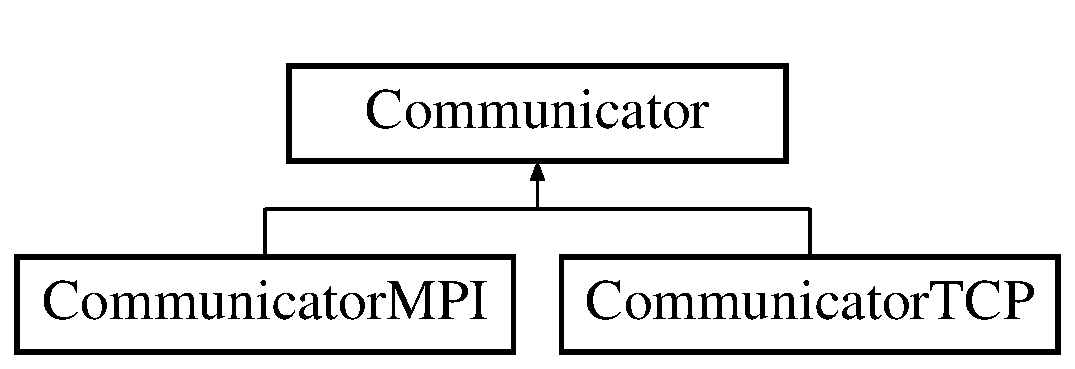
\includegraphics[height=2.000000cm]{classCommunicator}
\end{center}
\end{figure}
\subsection*{Public Member Functions}
\begin{DoxyCompactItemize}
\item 
\hypertarget{classCommunicator_a92ad155222aeafd1e5b1bd129809c2e9}{{\bfseries Communicator} (int type\-\_\-)}\label{classCommunicator_a92ad155222aeafd1e5b1bd129809c2e9}

\item 
\hypertarget{classCommunicator_a0a90cca12dcfb5721e9ac334e79c8802}{virtual int {\bfseries send} (const char $\ast$buf, int count, M\-D\-I\-\_\-\-Datatype datatype)=0}\label{classCommunicator_a0a90cca12dcfb5721e9ac334e79c8802}

\item 
\hypertarget{classCommunicator_af8618383684b7f2e1cea1a40acd43a81}{virtual int {\bfseries recv} (char $\ast$buf, int count, M\-D\-I\-\_\-\-Datatype datatype)=0}\label{classCommunicator_af8618383684b7f2e1cea1a40acd43a81}

\end{DoxyCompactItemize}


The documentation for this class was generated from the following files\-:\begin{DoxyCompactItemize}
\item 
/home/tbarnes/mdi/molssi\-\_\-driver\-\_\-interface/molssi\-\_\-driver\-\_\-interface/\hyperlink{communicator_8h}{communicator.\-h}\item 
/home/tbarnes/mdi/molssi\-\_\-driver\-\_\-interface/molssi\-\_\-driver\-\_\-interface/\hyperlink{communicator_8cpp}{communicator.\-cpp}\end{DoxyCompactItemize}

\hypertarget{classCommunicatorMPI}{\section{Communicator\-M\-P\-I Class Reference}
\label{classCommunicatorMPI}\index{Communicator\-M\-P\-I@{Communicator\-M\-P\-I}}
}
Inheritance diagram for Communicator\-M\-P\-I\-:\begin{figure}[H]
\begin{center}
\leavevmode
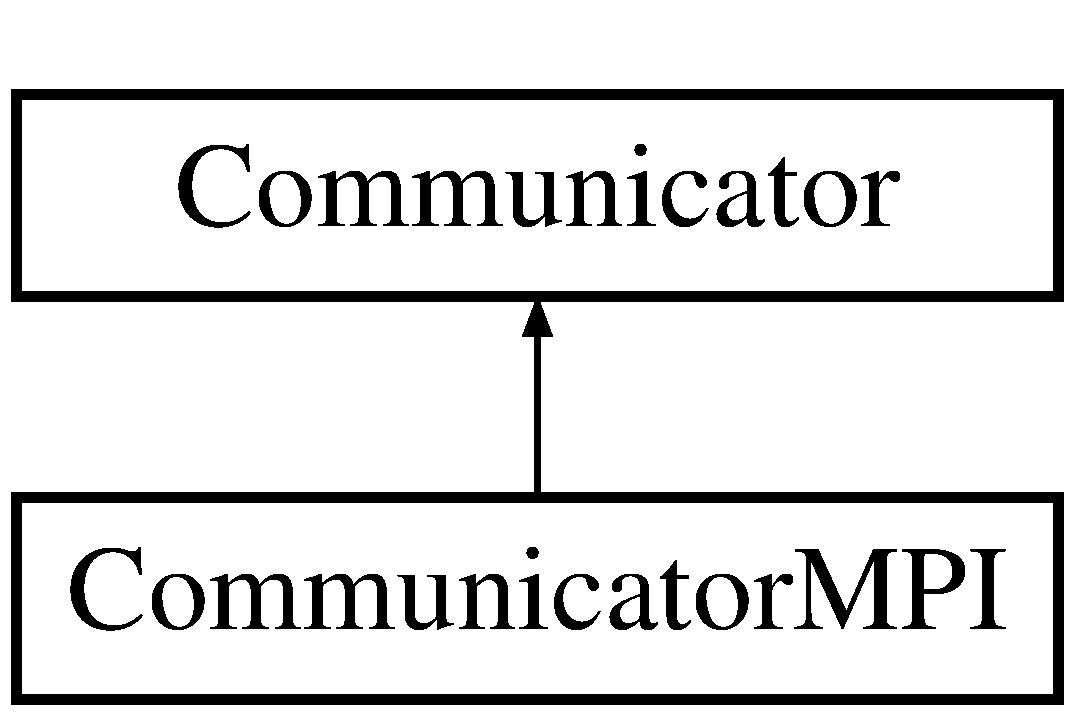
\includegraphics[height=2.000000cm]{classCommunicatorMPI}
\end{center}
\end{figure}
\subsection*{Public Member Functions}
\begin{DoxyCompactItemize}
\item 
\hypertarget{classCommunicatorMPI_aa07167a7e2dcebc0c9050ce1c18f3f32}{{\bfseries Communicator\-M\-P\-I} (int type\-\_\-, int mpi\-\_\-comm\-\_\-, int mpi\-\_\-rank\-\_\-)}\label{classCommunicatorMPI_aa07167a7e2dcebc0c9050ce1c18f3f32}

\item 
\hypertarget{classCommunicatorMPI_afd20883bec05ee4a5d97154a731a13cb}{int {\bfseries send} (const char $\ast$buf, int count, M\-D\-I\-\_\-\-Datatype datatype)}\label{classCommunicatorMPI_afd20883bec05ee4a5d97154a731a13cb}

\item 
\hypertarget{classCommunicatorMPI_ab0852541ca8f78fd3fc32e167386d76d}{int {\bfseries recv} (char $\ast$buf, int count, M\-D\-I\-\_\-\-Datatype datatype)}\label{classCommunicatorMPI_ab0852541ca8f78fd3fc32e167386d76d}

\end{DoxyCompactItemize}


The documentation for this class was generated from the following files\-:\begin{DoxyCompactItemize}
\item 
/home/tbarnes/mdi/molssi\-\_\-driver\-\_\-interface/molssi\-\_\-driver\-\_\-interface/\hyperlink{communicator_8h}{communicator.\-h}\item 
/home/tbarnes/mdi/molssi\-\_\-driver\-\_\-interface/molssi\-\_\-driver\-\_\-interface/\hyperlink{communicator_8cpp}{communicator.\-cpp}\end{DoxyCompactItemize}

\hypertarget{classCommunicatorTCP}{\section{Communicator\-T\-C\-P Class Reference}
\label{classCommunicatorTCP}\index{Communicator\-T\-C\-P@{Communicator\-T\-C\-P}}
}
Inheritance diagram for Communicator\-T\-C\-P\-:\begin{figure}[H]
\begin{center}
\leavevmode
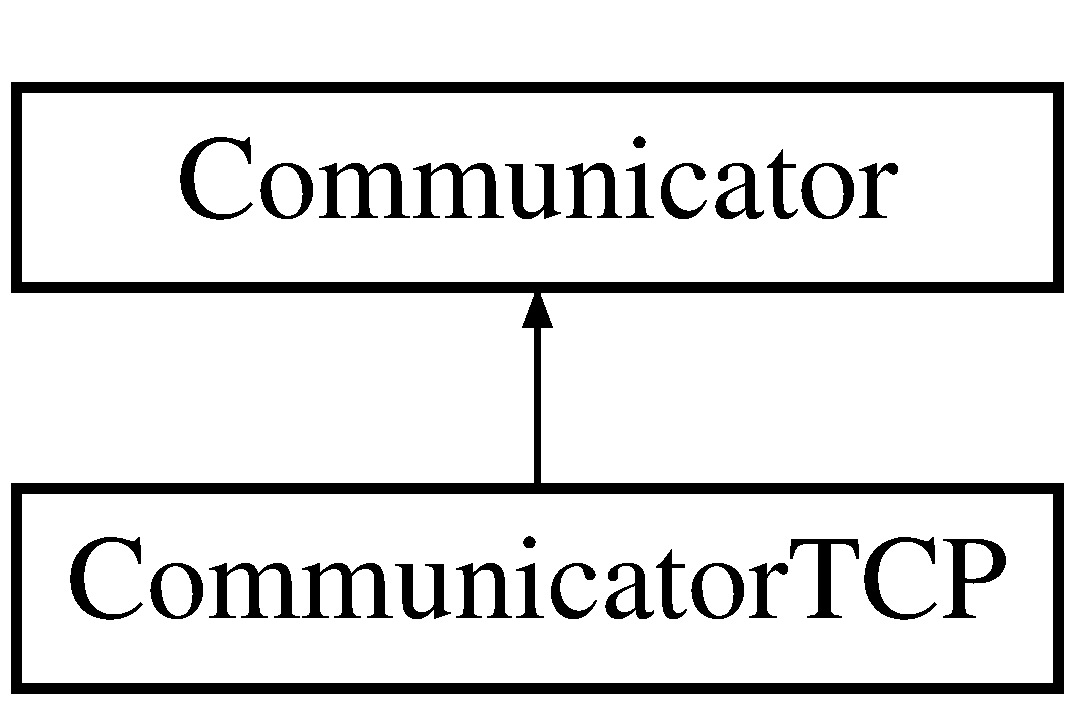
\includegraphics[height=2.000000cm]{classCommunicatorTCP}
\end{center}
\end{figure}
\subsection*{Public Member Functions}
\begin{DoxyCompactItemize}
\item 
\hypertarget{classCommunicatorTCP_a62b8536c01d0e5d3c7ab38df98a9a873}{{\bfseries Communicator\-T\-C\-P} (int type\-\_\-, int sockfd\-\_\-)}\label{classCommunicatorTCP_a62b8536c01d0e5d3c7ab38df98a9a873}

\item 
\hypertarget{classCommunicatorTCP_ac8e4894a12e34596ec7e78ab875933bf}{int {\bfseries send} (const char $\ast$buf, int count, M\-D\-I\-\_\-\-Datatype datatype)}\label{classCommunicatorTCP_ac8e4894a12e34596ec7e78ab875933bf}

\item 
\hypertarget{classCommunicatorTCP_a69d90c24e7bee5736c634565bdebab0d}{int {\bfseries recv} (char $\ast$buf, int count, M\-D\-I\-\_\-\-Datatype datatype)}\label{classCommunicatorTCP_a69d90c24e7bee5736c634565bdebab0d}

\end{DoxyCompactItemize}


The documentation for this class was generated from the following files\-:\begin{DoxyCompactItemize}
\item 
/home/tbarnes/mdi/molssi\-\_\-driver\-\_\-interface/molssi\-\_\-driver\-\_\-interface/\hyperlink{communicator_8h}{communicator.\-h}\item 
/home/tbarnes/mdi/molssi\-\_\-driver\-\_\-interface/molssi\-\_\-driver\-\_\-interface/\hyperlink{communicator_8cpp}{communicator.\-cpp}\end{DoxyCompactItemize}

\hypertarget{classmdi}{\section{mdi Module Reference}
\label{classmdi}\index{mdi@{mdi}}
}
\subsection*{Data Types}
\begin{DoxyCompactItemize}
\item 
interface \hyperlink{interfacemdi_1_1MDI__Accept__Communicator__}{M\-D\-I\-\_\-\-Accept\-\_\-\-Communicator\-\_\-}
\item 
interface \hyperlink{interfacemdi_1_1MDI__Init__}{M\-D\-I\-\_\-\-Init\-\_\-}
\item 
interface \hyperlink{interfacemdi_1_1MDI__MPI__Comm__}{M\-D\-I\-\_\-\-M\-P\-I\-\_\-\-Comm\-\_\-}
\item 
interface \hyperlink{interfacemdi_1_1mdi__recv}{mdi\-\_\-recv}
\item 
interface \hyperlink{interfacemdi_1_1MDI__Recv__}{M\-D\-I\-\_\-\-Recv\-\_\-}
\item 
interface \hyperlink{interfacemdi_1_1MDI__Recv__Command__}{M\-D\-I\-\_\-\-Recv\-\_\-\-Command\-\_\-}
\item 
interface \hyperlink{interfacemdi_1_1mdi__send}{mdi\-\_\-send}
\item 
interface \hyperlink{interfacemdi_1_1MDI__Send__}{M\-D\-I\-\_\-\-Send\-\_\-}
\item 
interface \hyperlink{interfacemdi_1_1MDI__Send__Command__}{M\-D\-I\-\_\-\-Send\-\_\-\-Command\-\_\-}
\end{DoxyCompactItemize}
\subsection*{Public Member Functions}
\begin{DoxyCompactItemize}
\item 
\hypertarget{classmdi_a35894bce734c441b9937f571436443b9}{subroutine {\bfseries mdi\-\_\-init} (foptions, fworld\-\_\-comm, ierr)}\label{classmdi_a35894bce734c441b9937f571436443b9}

\item 
\hypertarget{classmdi_a614089c34c2781079993f86374ee6d93}{subroutine {\bfseries mdi\-\_\-accept\-\_\-communicator} (\hyperlink{structcommunicator__struct}{communicator})}\label{classmdi_a614089c34c2781079993f86374ee6d93}

\item 
\hypertarget{classmdi_a127a7303cd7217c0d0d646e10b188f39}{subroutine {\bfseries mdi\-\_\-mpi\-\_\-comm} (comm, ierr)}\label{classmdi_a127a7303cd7217c0d0d646e10b188f39}

\item 
\hypertarget{classmdi_a83a8409162740c37f82776526e19d4cf}{subroutine {\bfseries mdi\-\_\-send\-\_\-s} (fstring, len, type, sockfd, ierr)}\label{classmdi_a83a8409162740c37f82776526e19d4cf}

\item 
\hypertarget{classmdi_ad5a7755632e8712b6d5609e2486b184a}{subroutine {\bfseries mdi\-\_\-send\-\_\-d} (fdata, len, type, sockfd, ierr)}\label{classmdi_ad5a7755632e8712b6d5609e2486b184a}

\item 
\hypertarget{classmdi_a57bcbe45a8445f19b02126f904b43774}{subroutine {\bfseries mdi\-\_\-send\-\_\-dv} (fdata, len, type, sockfd, ierr)}\label{classmdi_a57bcbe45a8445f19b02126f904b43774}

\item 
\hypertarget{classmdi_a9451f9ead8226273424cb7efbef245c3}{subroutine {\bfseries mdi\-\_\-send\-\_\-i} (fdata, len, type, sockfd, ierr)}\label{classmdi_a9451f9ead8226273424cb7efbef245c3}

\item 
\hypertarget{classmdi_add16db0836d8e0f3cfe310e175e8243c}{subroutine {\bfseries mdi\-\_\-send\-\_\-iv} (fdata, len, type, sockfd, ierr)}\label{classmdi_add16db0836d8e0f3cfe310e175e8243c}

\item 
\hypertarget{classmdi_a78af4fc262563d2d8820a3a7cbfe0a92}{subroutine {\bfseries mdi\-\_\-recv\-\_\-s} (fstring, len, type, sockfd, ierr)}\label{classmdi_a78af4fc262563d2d8820a3a7cbfe0a92}

\item 
\hypertarget{classmdi_a557c30482625b71f46ee392d70426014}{subroutine {\bfseries mdi\-\_\-recv\-\_\-d} (fdata, len, type, sockfd, ierr)}\label{classmdi_a557c30482625b71f46ee392d70426014}

\item 
\hypertarget{classmdi_a66dc1c9e1462e5c53bd36c720aa12a38}{subroutine {\bfseries mdi\-\_\-recv\-\_\-dv} (fdata, len, type, sockfd, ierr)}\label{classmdi_a66dc1c9e1462e5c53bd36c720aa12a38}

\item 
\hypertarget{classmdi_a50204266766bbd60ec46f697309b9c5c}{subroutine {\bfseries mdi\-\_\-recv\-\_\-i} (fdata, len, type, sockfd, ierr)}\label{classmdi_a50204266766bbd60ec46f697309b9c5c}

\item 
\hypertarget{classmdi_adb59292b64be533922c3bd55c04df653}{subroutine {\bfseries mdi\-\_\-recv\-\_\-iv} (fdata, len, type, sockfd, ierr)}\label{classmdi_adb59292b64be533922c3bd55c04df653}

\item 
\hypertarget{classmdi_a9b4dc2e960271e8779e842b9e1edc0dd}{subroutine {\bfseries mdi\-\_\-send\-\_\-command} (fstring, sockfd, ierr)}\label{classmdi_a9b4dc2e960271e8779e842b9e1edc0dd}

\item 
\hypertarget{classmdi_a3a3b366cde72e01a9d3a928e902e58d0}{subroutine {\bfseries mdi\-\_\-recv\-\_\-command} (fstring, sockfd, ierr)}\label{classmdi_a3a3b366cde72e01a9d3a928e902e58d0}

\end{DoxyCompactItemize}
\subsection*{Public Attributes}
\begin{DoxyCompactItemize}
\item 
\hypertarget{classmdi_accae5b01e087f8738d86006e68417f6d}{integer, dimension(c, name=\char`\"{}mdi\-\_\-kelvin\-\_\-to\-\_\-hartree\char`\"{}), \\*
protected {\bfseries bind}}\label{classmdi_accae5b01e087f8738d86006e68417f6d}

\item 
\hypertarget{classmdi_a476a171077b89b7bc1e0153edaee118a}{integer, protected {\bfseries mdi\-\_\-command\-\_\-length}}\label{classmdi_a476a171077b89b7bc1e0153edaee118a}

\item 
\hypertarget{classmdi_a8038fa45863d082fafb692e8bc1f4b5a}{integer, protected {\bfseries mdi\-\_\-name\-\_\-length}}\label{classmdi_a8038fa45863d082fafb692e8bc1f4b5a}

\item 
\hypertarget{classmdi_ae85ef43174229bd688543ad4bcc08a2b}{integer, protected {\bfseries mdi\-\_\-int}}\label{classmdi_ae85ef43174229bd688543ad4bcc08a2b}

\item 
\hypertarget{classmdi_a69ba399f9ad46c8ac033b26574c9b6ef}{integer, protected {\bfseries mdi\-\_\-double}}\label{classmdi_a69ba399f9ad46c8ac033b26574c9b6ef}

\item 
\hypertarget{classmdi_a5741adbde5b79f06a9b94b17c7f16eb7}{integer, protected {\bfseries mdi\-\_\-char}}\label{classmdi_a5741adbde5b79f06a9b94b17c7f16eb7}

\item 
\hypertarget{classmdi_a1605c457efb88fc7e1f169734c58b52c}{integer, protected {\bfseries mdi\-\_\-tcp}}\label{classmdi_a1605c457efb88fc7e1f169734c58b52c}

\item 
\hypertarget{classmdi_a4039d7ab89098798e98dda20ece81eaf}{integer, protected {\bfseries mdi\-\_\-mpi}}\label{classmdi_a4039d7ab89098798e98dda20ece81eaf}

\item 
\hypertarget{classmdi_aff013df9c91a218d860486ff0fc757e4}{real(kind=8), dimension(c, \\*
name=\char`\"{}mdi\-\_\-kelvin\-\_\-to\-\_\-hartree\char`\"{}), \\*
protected {\bfseries bind}}\label{classmdi_aff013df9c91a218d860486ff0fc757e4}

\item 
\hypertarget{classmdi_af74f78803c251e23cd5022a8df7abc1e}{real(kind=8), protected {\bfseries mdi\-\_\-meter\-\_\-to\-\_\-bohr}}\label{classmdi_af74f78803c251e23cd5022a8df7abc1e}

\item 
\hypertarget{classmdi_a6abac217d729188855210e9327333578}{real(kind=8), protected {\bfseries mdi\-\_\-angstrom\-\_\-to\-\_\-bohr}}\label{classmdi_a6abac217d729188855210e9327333578}

\item 
\hypertarget{classmdi_a583e3421719bbf0bd951f455a0032766}{real(kind=8), protected {\bfseries mdi\-\_\-second\-\_\-to\-\_\-aut}}\label{classmdi_a583e3421719bbf0bd951f455a0032766}

\item 
\hypertarget{classmdi_ad350838a7aea84b6eca15da72d3ee4fc}{real(kind=8), protected {\bfseries mdi\-\_\-picosecond\-\_\-to\-\_\-aut}}\label{classmdi_ad350838a7aea84b6eca15da72d3ee4fc}

\item 
\hypertarget{classmdi_ace10d5db76cf54244d54b62e77b9d9a6}{real(kind=8), protected {\bfseries mdi\-\_\-newton\-\_\-to\-\_\-auf}}\label{classmdi_ace10d5db76cf54244d54b62e77b9d9a6}

\item 
\hypertarget{classmdi_a0b4e777d36fe90d506f70b16abb1b910}{real(kind=8), protected {\bfseries mdi\-\_\-joule\-\_\-to\-\_\-hartree}}\label{classmdi_a0b4e777d36fe90d506f70b16abb1b910}

\item 
\hypertarget{classmdi_a12a5c4e648f84d60dd261349d5e2cf37}{real(kind=8), protected {\bfseries mdi\-\_\-kj\-\_\-to\-\_\-hartree}}\label{classmdi_a12a5c4e648f84d60dd261349d5e2cf37}

\item 
\hypertarget{classmdi_a761336e719b236672a145cf86a8b7c95}{real(kind=8), protected {\bfseries mdi\-\_\-kjpermol\-\_\-to\-\_\-hartree}}\label{classmdi_a761336e719b236672a145cf86a8b7c95}

\item 
\hypertarget{classmdi_a2a5635f450c619dabb104846fd972b22}{real(kind=8), protected {\bfseries mdi\-\_\-kcalpermol\-\_\-to\-\_\-hartree}}\label{classmdi_a2a5635f450c619dabb104846fd972b22}

\item 
\hypertarget{classmdi_a02fe8f5658dc9d6379ceb2cc40b24b56}{real(kind=8), protected {\bfseries mdi\-\_\-ev\-\_\-to\-\_\-hartree}}\label{classmdi_a02fe8f5658dc9d6379ceb2cc40b24b56}

\item 
\hypertarget{classmdi_a4eefaa8b0fe9c708b1ba69ae86bac95c}{real(kind=8), protected {\bfseries mdi\-\_\-rydberg\-\_\-to\-\_\-hartree}}\label{classmdi_a4eefaa8b0fe9c708b1ba69ae86bac95c}

\item 
\hypertarget{classmdi_a5fc09af33b0b858f96014b3f9fdd7ee5}{real(kind=8), protected {\bfseries mdi\-\_\-kelvin\-\_\-to\-\_\-hartree}}\label{classmdi_a5fc09af33b0b858f96014b3f9fdd7ee5}

\end{DoxyCompactItemize}


The documentation for this module was generated from the following file\-:\begin{DoxyCompactItemize}
\item 
/home/tbarnes/mdi/molssi\-\_\-driver\-\_\-interface/molssi\-\_\-driver\-\_\-interface/mdi\-\_\-f90.\-f90\end{DoxyCompactItemize}

\hypertarget{interfacemdi_1_1MDI__Accept__Communicator__}{\section{mdi\-:\-:M\-D\-I\-\_\-\-Accept\-\_\-\-Communicator\-\_\- Interface Reference}
\label{interfacemdi_1_1MDI__Accept__Communicator__}\index{mdi\-::\-M\-D\-I\-\_\-\-Accept\-\_\-\-Communicator\-\_\-@{mdi\-::\-M\-D\-I\-\_\-\-Accept\-\_\-\-Communicator\-\_\-}}
}
\subsection*{Public Member Functions}
\begin{DoxyCompactItemize}
\item 
\hypertarget{interfacemdi_1_1MDI__Accept__Communicator___af692624300292e68edf192a9379e4182}{integer(kind=c\-\_\-int) function {\bfseries mdi\-\_\-accept\-\_\-communicator\-\_\-} ()}\label{interfacemdi_1_1MDI__Accept__Communicator___af692624300292e68edf192a9379e4182}

\end{DoxyCompactItemize}


The documentation for this interface was generated from the following file\-:\begin{DoxyCompactItemize}
\item 
/home/tbarnes/mdi/molssi\-\_\-driver\-\_\-interface/molssi\-\_\-driver\-\_\-interface/mdi\-\_\-f90.\-f90\end{DoxyCompactItemize}

\hypertarget{interfacemdi_1_1MDI__Conversion__Factor__}{}\doxysection{mdi\+::M\+D\+I\+\_\+\+Conversion\+\_\+\+Factor\+\_\+ Interface Reference}
\label{interfacemdi_1_1MDI__Conversion__Factor__}\index{mdi::MDI\_Conversion\_Factor\_@{mdi::MDI\_Conversion\_Factor\_}}
\doxysubsection*{Public Member Functions}
\begin{DoxyCompactItemize}
\item 
\mbox{\Hypertarget{interfacemdi_1_1MDI__Conversion__Factor___acad6a9822471076622182f03b6073c77}\label{interfacemdi_1_1MDI__Conversion__Factor___acad6a9822471076622182f03b6073c77}} 
real(kind=c\+\_\+double) function {\bfseries mdi\+\_\+conversion\+\_\+factor\+\_\+} (in\+\_\+unit, out\+\_\+unit)
\end{DoxyCompactItemize}


The documentation for this interface was generated from the following file\+:\begin{DoxyCompactItemize}
\item 
/\+Users/tbarnes/\+Documents/mdi/\+M\+D\+I\+\_\+\+Library/\+M\+D\+I\+\_\+\+Library/mdi\+\_\+f90.\+f90\end{DoxyCompactItemize}

\hypertarget{interfacemdi_1_1MDI__Init__}{\section{mdi\-:\-:M\-D\-I\-\_\-\-Init\-\_\- Interface Reference}
\label{interfacemdi_1_1MDI__Init__}\index{mdi\-::\-M\-D\-I\-\_\-\-Init\-\_\-@{mdi\-::\-M\-D\-I\-\_\-\-Init\-\_\-}}
}
\subsection*{Public Member Functions}
\begin{DoxyCompactItemize}
\item 
\hypertarget{interfacemdi_1_1MDI__Init___a6d3a67f8175464baa0a4e54caecfa2ae}{integer(kind=c\-\_\-int) function {\bfseries mdi\-\_\-init\-\_\-} (options, world\-\_\-comm)}\label{interfacemdi_1_1MDI__Init___a6d3a67f8175464baa0a4e54caecfa2ae}

\end{DoxyCompactItemize}


The documentation for this interface was generated from the following file\-:\begin{DoxyCompactItemize}
\item 
/home/tbarnes/mdi/molssi\-\_\-driver\-\_\-interface/molssi\-\_\-driver\-\_\-interface/mdi\-\_\-f90.\-f90\end{DoxyCompactItemize}

\hypertarget{interfacemdi_1_1mdi__recv}{}\doxysection{mdi\+::mdi\+\_\+recv Interface Reference}
\label{interfacemdi_1_1mdi__recv}\index{mdi::mdi\_recv@{mdi::mdi\_recv}}
\doxysubsection*{Public Member Functions}
\begin{DoxyCompactItemize}
\item 
\mbox{\Hypertarget{interfacemdi_1_1mdi__recv_a7311db44b9a07e51819c43cdb4a454bf}\label{interfacemdi_1_1mdi__recv_a7311db44b9a07e51819c43cdb4a454bf}} 
subroutine {\bfseries mdi\+\_\+recv\+\_\+s} (fbuf, count, datatype, comm, ierr)
\item 
\mbox{\Hypertarget{interfacemdi_1_1mdi__recv_ac0a9b1a924c7106d0a574e15a5882291}\label{interfacemdi_1_1mdi__recv_ac0a9b1a924c7106d0a574e15a5882291}} 
subroutine {\bfseries mdi\+\_\+recv\+\_\+d} (fbuf, count, datatype, comm, ierr)
\item 
\mbox{\Hypertarget{interfacemdi_1_1mdi__recv_ad5fc789a537ac5781f5d2590d7cd34d5}\label{interfacemdi_1_1mdi__recv_ad5fc789a537ac5781f5d2590d7cd34d5}} 
subroutine {\bfseries mdi\+\_\+recv\+\_\+dv} (fbuf, count, datatype, comm, ierr)
\item 
\mbox{\Hypertarget{interfacemdi_1_1mdi__recv_a026f22dc4ed36c50764c7dc2cdfe9bd1}\label{interfacemdi_1_1mdi__recv_a026f22dc4ed36c50764c7dc2cdfe9bd1}} 
subroutine {\bfseries mdi\+\_\+recv\+\_\+i} (fbuf, count, datatype, comm, ierr)
\item 
\mbox{\Hypertarget{interfacemdi_1_1mdi__recv_abe214d15e6c082d38999a36fb8d33fea}\label{interfacemdi_1_1mdi__recv_abe214d15e6c082d38999a36fb8d33fea}} 
subroutine {\bfseries mdi\+\_\+recv\+\_\+iv} (fbuf, count, datatype, comm, ierr)
\end{DoxyCompactItemize}


The documentation for this interface was generated from the following file\+:\begin{DoxyCompactItemize}
\item 
/\+Users/tbarnes/\+Documents/mdi/\+M\+D\+I\+\_\+\+Library/\+M\+D\+I\+\_\+\+Library/mdi\+\_\+f90.\+f90\end{DoxyCompactItemize}

\hypertarget{interfacemdi_1_1MDI__Recv__}{}\doxysection{mdi\+::M\+D\+I\+\_\+\+Recv\+\_\+ Interface Reference}
\label{interfacemdi_1_1MDI__Recv__}\index{mdi::MDI\_Recv\_@{mdi::MDI\_Recv\_}}
\doxysubsection*{Public Member Functions}
\begin{DoxyCompactItemize}
\item 
\mbox{\Hypertarget{interfacemdi_1_1MDI__Recv___a8a02f4e2009b1219ed101b4b2c2584ed}\label{interfacemdi_1_1MDI__Recv___a8a02f4e2009b1219ed101b4b2c2584ed}} 
integer(kind=c\+\_\+int) function {\bfseries mdi\+\_\+recv\+\_\+} (buf, count, datatype, comm)
\end{DoxyCompactItemize}


The documentation for this interface was generated from the following file\+:\begin{DoxyCompactItemize}
\item 
/\+Users/tbarnes/\+Documents/mdi/\+M\+D\+I\+\_\+\+Library/\+M\+D\+I\+\_\+\+Library/mdi\+\_\+f90.\+f90\end{DoxyCompactItemize}

\hypertarget{interfacemdi_1_1MDI__Recv__Command__}{}\doxysection{mdi\+::M\+D\+I\+\_\+\+Recv\+\_\+\+Command\+\_\+ Interface Reference}
\label{interfacemdi_1_1MDI__Recv__Command__}\index{mdi::MDI\_Recv\_Command\_@{mdi::MDI\_Recv\_Command\_}}
\doxysubsection*{Public Member Functions}
\begin{DoxyCompactItemize}
\item 
\mbox{\Hypertarget{interfacemdi_1_1MDI__Recv__Command___a22b67734eebe9ccf72cd71a8894c28e4}\label{interfacemdi_1_1MDI__Recv__Command___a22b67734eebe9ccf72cd71a8894c28e4}} 
integer(kind=c\+\_\+int) function {\bfseries mdi\+\_\+recv\+\_\+command\+\_\+} (buf, comm)
\end{DoxyCompactItemize}


The documentation for this interface was generated from the following file\+:\begin{DoxyCompactItemize}
\item 
/\+Users/tbarnes/\+Documents/mdi/\+M\+D\+I\+\_\+\+Library/\+M\+D\+I\+\_\+\+Library/mdi\+\_\+f90.\+f90\end{DoxyCompactItemize}

\hypertarget{interfacemdi_1_1mdi__send}{\section{mdi\-:\-:mdi\-\_\-send Interface Reference}
\label{interfacemdi_1_1mdi__send}\index{mdi\-::mdi\-\_\-send@{mdi\-::mdi\-\_\-send}}
}
\subsection*{Public Member Functions}
\begin{DoxyCompactItemize}
\item 
\hypertarget{interfacemdi_1_1mdi__send_a3ddadb7d7d6c6c71986251adc8658fb7}{subroutine {\bfseries mdi\-\_\-send\-\_\-s} (fstring, len, type, sockfd, ierr)}\label{interfacemdi_1_1mdi__send_a3ddadb7d7d6c6c71986251adc8658fb7}

\item 
\hypertarget{interfacemdi_1_1mdi__send_af2e36516f7aaa3233d73305279d81504}{subroutine {\bfseries mdi\-\_\-send\-\_\-d} (fdata, len, type, sockfd, ierr)}\label{interfacemdi_1_1mdi__send_af2e36516f7aaa3233d73305279d81504}

\item 
\hypertarget{interfacemdi_1_1mdi__send_a4353240dcf91e1081c3f8c8b6093258e}{subroutine {\bfseries mdi\-\_\-send\-\_\-dv} (fdata, len, type, sockfd, ierr)}\label{interfacemdi_1_1mdi__send_a4353240dcf91e1081c3f8c8b6093258e}

\item 
\hypertarget{interfacemdi_1_1mdi__send_aa33ab4f1c856362420d6319d61e49806}{subroutine {\bfseries mdi\-\_\-send\-\_\-i} (fdata, len, type, sockfd, ierr)}\label{interfacemdi_1_1mdi__send_aa33ab4f1c856362420d6319d61e49806}

\item 
\hypertarget{interfacemdi_1_1mdi__send_a6b75e458ac31ee62040de3c1487d372a}{subroutine {\bfseries mdi\-\_\-send\-\_\-iv} (fdata, len, type, sockfd, ierr)}\label{interfacemdi_1_1mdi__send_a6b75e458ac31ee62040de3c1487d372a}

\end{DoxyCompactItemize}


The documentation for this interface was generated from the following file\-:\begin{DoxyCompactItemize}
\item 
/home/tbarnes/mdi/molssi\-\_\-driver\-\_\-interface/molssi\-\_\-driver\-\_\-interface/mdi\-\_\-f90.\-f90\end{DoxyCompactItemize}

\hypertarget{interfacemdi_1_1MDI__Send__}{\section{mdi\-:\-:M\-D\-I\-\_\-\-Send\-\_\- Interface Reference}
\label{interfacemdi_1_1MDI__Send__}\index{mdi\-::\-M\-D\-I\-\_\-\-Send\-\_\-@{mdi\-::\-M\-D\-I\-\_\-\-Send\-\_\-}}
}
\subsection*{Public Member Functions}
\begin{DoxyCompactItemize}
\item 
\hypertarget{interfacemdi_1_1MDI__Send___a56b7aefaad39a2e38c76f253fdf76a6b}{integer(kind=c\-\_\-int) function {\bfseries mdi\-\_\-send\-\_\-} (buf, count, datatype, comm)}\label{interfacemdi_1_1MDI__Send___a56b7aefaad39a2e38c76f253fdf76a6b}

\end{DoxyCompactItemize}


The documentation for this interface was generated from the following file\-:\begin{DoxyCompactItemize}
\item 
/home/tbarnes/mdi/molssi\-\_\-driver\-\_\-interface/molssi\-\_\-driver\-\_\-interface/mdi\-\_\-f90.\-f90\end{DoxyCompactItemize}

\hypertarget{interfacemdi_1_1MDI__Send__Command__}{}\doxysection{mdi\+::M\+D\+I\+\_\+\+Send\+\_\+\+Command\+\_\+ Interface Reference}
\label{interfacemdi_1_1MDI__Send__Command__}\index{mdi::MDI\_Send\_Command\_@{mdi::MDI\_Send\_Command\_}}
\doxysubsection*{Public Member Functions}
\begin{DoxyCompactItemize}
\item 
\mbox{\Hypertarget{interfacemdi_1_1MDI__Send__Command___ad79374503988a8b76342367a2b38feb5}\label{interfacemdi_1_1MDI__Send__Command___ad79374503988a8b76342367a2b38feb5}} 
integer(kind=c\+\_\+int) function {\bfseries mdi\+\_\+send\+\_\+command\+\_\+} (buf, comm)
\end{DoxyCompactItemize}


The documentation for this interface was generated from the following file\+:\begin{DoxyCompactItemize}
\item 
/\+Users/tbarnes/\+Documents/mdi/\+M\+D\+I\+\_\+\+Library/\+M\+D\+I\+\_\+\+Library/mdi\+\_\+f90.\+f90\end{DoxyCompactItemize}

\chapter{File Documentation}
\hypertarget{communicator_8cpp}{\section{/home/tbarnes/mdi/molssi\-\_\-driver\-\_\-interface/molssi\-\_\-driver\-\_\-interface/communicator.cpp File Reference}
\label{communicator_8cpp}\index{/home/tbarnes/mdi/molssi\-\_\-driver\-\_\-interface/molssi\-\_\-driver\-\_\-interface/communicator.\-cpp@{/home/tbarnes/mdi/molssi\-\_\-driver\-\_\-interface/molssi\-\_\-driver\-\_\-interface/communicator.\-cpp}}
}


Class definition for handling communication between connect codes.  


{\ttfamily \#include $<$mpi.\-h$>$}\\*
{\ttfamily \#include $<$stdio.\-h$>$}\\*
{\ttfamily \#include $<$stdlib.\-h$>$}\\*
{\ttfamily \#include $<$unistd.\-h$>$}\\*
{\ttfamily \#include \char`\"{}mdi.\-h\char`\"{}}\\*
{\ttfamily \#include \char`\"{}communicator.\-h\char`\"{}}\\*
\subsection*{Variables}
\begin{DoxyCompactItemize}
\item 
\hypertarget{communicator_8cpp_a1806a2b57b24b2dd653eb4475758e5d2}{vector$<$ \hyperlink{classCommunicator}{Communicator} $\ast$ $>$ {\bfseries communicators}}\label{communicator_8cpp_a1806a2b57b24b2dd653eb4475758e5d2}

\end{DoxyCompactItemize}


\subsection{Detailed Description}
Class definition for handling communication between connect codes. 
\hypertarget{communicator_8h}{}\doxysection{/\+Users/tbarnes/\+Documents/mdi/\+M\+D\+I\+\_\+\+Library/\+M\+D\+I\+\_\+\+Library/communicator.h File Reference}
\label{communicator_8h}\index{/Users/tbarnes/Documents/mdi/MDI\_Library/MDI\_Library/communicator.h@{/Users/tbarnes/Documents/mdi/MDI\_Library/MDI\_Library/communicator.h}}


Class declaration for handling communication between connected codes.  


{\ttfamily \#include $<$mpi.\+h$>$}\newline
{\ttfamily \#include \char`\"{}mdi.\+h\char`\"{}}\newline
\doxysubsection*{Classes}
\begin{DoxyCompactItemize}
\item 
struct \mbox{\hyperlink{structcommunicator__struct}{communicator\+\_\+struct}}
\item 
struct \mbox{\hyperlink{structdynamic__array__struct}{dynamic\+\_\+array\+\_\+struct}}
\end{DoxyCompactItemize}
\doxysubsection*{Typedefs}
\begin{DoxyCompactItemize}
\item 
\mbox{\Hypertarget{communicator_8h_a7f1369263a8fc2bfc5c3f69302d4dea7}\label{communicator_8h_a7f1369263a8fc2bfc5c3f69302d4dea7}} 
typedef struct \mbox{\hyperlink{structcommunicator__struct}{communicator\+\_\+struct}} {\bfseries communicator}
\item 
\mbox{\Hypertarget{communicator_8h_ae301b80284ed481523c43e095398ba92}\label{communicator_8h_ae301b80284ed481523c43e095398ba92}} 
typedef struct \mbox{\hyperlink{structdynamic__array__struct}{dynamic\+\_\+array\+\_\+struct}} {\bfseries vector}
\end{DoxyCompactItemize}
\doxysubsection*{Functions}
\begin{DoxyCompactItemize}
\item 
\mbox{\Hypertarget{communicator_8h_a6c749e461a84e471bcab02d8115a1dfa}\label{communicator_8h_a6c749e461a84e471bcab02d8115a1dfa}} 
int {\bfseries vector\+\_\+init} (\mbox{\hyperlink{structdynamic__array__struct}{vector}} $\ast$v, size\+\_\+t stride)
\item 
\mbox{\Hypertarget{communicator_8h_a53e2a90f50c539f8239225d6f39c0213}\label{communicator_8h_a53e2a90f50c539f8239225d6f39c0213}} 
int {\bfseries vector\+\_\+push\+\_\+back} (\mbox{\hyperlink{structdynamic__array__struct}{vector}} $\ast$v, void $\ast$element)
\item 
\mbox{\Hypertarget{communicator_8h_a75ffb2ad4233613bd0c97d40b1c68611}\label{communicator_8h_a75ffb2ad4233613bd0c97d40b1c68611}} 
void $\ast$ {\bfseries vector\+\_\+get} (\mbox{\hyperlink{structdynamic__array__struct}{vector}} $\ast$v, int index)
\item 
\mbox{\Hypertarget{communicator_8h_ad3c615060f602d600023a678acee7e28}\label{communicator_8h_ad3c615060f602d600023a678acee7e28}} 
int {\bfseries communicator\+\_\+send} (const void $\ast$buf, int count, M\+D\+I\+\_\+\+Datatype datatype, M\+D\+I\+\_\+\+Comm comm)
\item 
\mbox{\Hypertarget{communicator_8h_a309565fdcf2cdb4a779edef5787e6fa9}\label{communicator_8h_a309565fdcf2cdb4a779edef5787e6fa9}} 
int {\bfseries communicator\+\_\+recv} (void $\ast$buf, int count, M\+D\+I\+\_\+\+Datatype datatype, M\+D\+I\+\_\+\+Comm comm)
\end{DoxyCompactItemize}
\doxysubsection*{Variables}
\begin{DoxyCompactItemize}
\item 
\mbox{\Hypertarget{communicator_8h_aae895626c3da244edb20b7ffcca7d05f}\label{communicator_8h_aae895626c3da244edb20b7ffcca7d05f}} 
\mbox{\hyperlink{structdynamic__array__struct}{vector}} {\bfseries communicators}
\end{DoxyCompactItemize}


\doxysubsection{Detailed Description}
Class declaration for handling communication between connected codes. 


\hypertarget{mdi_8cpp}{\section{/home/tbarnes/mdi/molssi\-\_\-driver\-\_\-interface/molssi\-\_\-driver\-\_\-interface/mdi.cpp File Reference}
\label{mdi_8cpp}\index{/home/tbarnes/mdi/molssi\-\_\-driver\-\_\-interface/molssi\-\_\-driver\-\_\-interface/mdi.\-cpp@{/home/tbarnes/mdi/molssi\-\_\-driver\-\_\-interface/molssi\-\_\-driver\-\_\-interface/mdi.\-cpp}}
}


Functions callable by users of the Mol\-S\-S\-I Driver Interface.  


{\ttfamily \#include $<$signal.\-h$>$}\\*
{\ttfamily \#include $<$netdb.\-h$>$}\\*
{\ttfamily \#include $<$netinet/in.\-h$>$}\\*
{\ttfamily \#include $<$stdio.\-h$>$}\\*
{\ttfamily \#include $<$stdlib.\-h$>$}\\*
{\ttfamily \#include $<$string.\-h$>$}\\*
{\ttfamily \#include $<$sys/socket.\-h$>$}\\*
{\ttfamily \#include $<$sys/types.\-h$>$}\\*
{\ttfamily \#include $<$sys/un.\-h$>$}\\*
{\ttfamily \#include $<$unistd.\-h$>$}\\*
{\ttfamily \#include $<$errno.\-h$>$}\\*
{\ttfamily \#include $<$iostream$>$}\\*
{\ttfamily \#include $<$vector$>$}\\*
{\ttfamily \#include \char`\"{}mdi.\-h\char`\"{}}\\*
\subsection*{Classes}
\begin{DoxyCompactItemize}
\item 
struct \hyperlink{structcommunicator__struct}{communicator\-\_\-struct}
\end{DoxyCompactItemize}
\subsection*{Macros}
\begin{DoxyCompactItemize}
\item 
\hypertarget{mdi_8cpp_a272bfb6c5307fb3f4c40336dce06ef75}{\#define {\bfseries M\-D\-I\-\_\-\-N\-A\-M\-E\-\_\-\-L\-E\-N\-G\-T\-H\-\_\-\-I\-N\-T\-E\-R\-N\-A\-L}~12}\label{mdi_8cpp_a272bfb6c5307fb3f4c40336dce06ef75}

\end{DoxyCompactItemize}
\subsection*{Typedefs}
\begin{DoxyCompactItemize}
\item 
\hypertarget{mdi_8cpp_a7f1369263a8fc2bfc5c3f69302d4dea7}{typedef struct \hyperlink{structcommunicator__struct}{communicator\-\_\-struct} {\bfseries communicator}}\label{mdi_8cpp_a7f1369263a8fc2bfc5c3f69302d4dea7}

\end{DoxyCompactItemize}
\subsection*{Functions}
\begin{DoxyCompactItemize}
\item 
\hypertarget{mdi_8cpp_a10ceefc902b8eb71e2383d7ac95de2c7}{void {\bfseries mdi\-\_\-error} (const char $\ast$message)}\label{mdi_8cpp_a10ceefc902b8eb71e2383d7ac95de2c7}

\item 
\hypertarget{mdi_8cpp_a47630f8f823b92ad9333c3c5f130cf90}{void {\bfseries sigint\-\_\-handler} (int dummy)}\label{mdi_8cpp_a47630f8f823b92ad9333c3c5f130cf90}

\item 
\hypertarget{mdi_8cpp_a8bdb67120e391198c5d7e592169a7e67}{int {\bfseries gather\-\_\-names} (const char $\ast$hostname\-\_\-ptr, bool do\-\_\-split)}\label{mdi_8cpp_a8bdb67120e391198c5d7e592169a7e67}

\item 
\hypertarget{mdi_8cpp_af15a7354cf37401b3a482614dedbcad9}{int {\bfseries M\-D\-I\-\_\-\-Listen\-\_\-\-T\-C\-P} (int port)}\label{mdi_8cpp_af15a7354cf37401b3a482614dedbcad9}

\item 
\hypertarget{mdi_8cpp_a200d815da834074e8a718519b9f833a6}{int {\bfseries M\-D\-I\-\_\-\-Request\-\_\-\-Connection\-\_\-\-T\-C\-P} (int port, char $\ast$hostname\-\_\-ptr)}\label{mdi_8cpp_a200d815da834074e8a718519b9f833a6}

\item 
int \hyperlink{mdi_8cpp_ae05ae377fa8de592f62c696c041b7d0a}{M\-D\-I\-\_\-\-Init} (const char $\ast$options, void $\ast$world\-\_\-comm)
\begin{DoxyCompactList}\small\item\em Initialize communication through the M\-D\-I library. \end{DoxyCompactList}\item 
int \hyperlink{mdi_8cpp_af13ac32549acde2f176447663449ae8d}{M\-D\-I\-\_\-\-Accept\-\_\-\-Communicator} ()
\begin{DoxyCompactList}\small\item\em Accept a new M\-D\-I communicator. \end{DoxyCompactList}\item 
int \hyperlink{mdi_8cpp_af186725e545bc894336d28aa18fdb89e}{M\-D\-I\-\_\-\-Send} (const char $\ast$buf, int count, int datatype, int comm)
\begin{DoxyCompactList}\small\item\em Send data through the M\-D\-I connection. \end{DoxyCompactList}\item 
int \hyperlink{mdi_8cpp_aa17b455a7e09fbb80224b726110979e6}{M\-D\-I\-\_\-\-Recv} (char $\ast$buf, int count, int datatype, int comm)
\begin{DoxyCompactList}\small\item\em Receive data through the M\-D\-I connection. \end{DoxyCompactList}\item 
int \hyperlink{mdi_8cpp_aea30c460e6369a77acc101437e94e87e}{M\-D\-I\-\_\-\-Send\-\_\-\-Command} (const char $\ast$buf, int comm)
\begin{DoxyCompactList}\small\item\em Send a command of length {\ttfamily M\-D\-I\-\_\-\-C\-O\-M\-M\-A\-N\-D\-\_\-\-L\-E\-N\-G\-T\-H} through the M\-D\-I connection. \end{DoxyCompactList}\item 
int \hyperlink{mdi_8cpp_a4a1d5d1b629bd53ee6f6099058f5b019}{M\-D\-I\-\_\-\-Recv\-\_\-\-Command} (char $\ast$buf, int comm)
\begin{DoxyCompactList}\small\item\em Receive a command of length {\ttfamily M\-D\-I\-\_\-\-C\-O\-M\-M\-A\-N\-D\-\_\-\-L\-E\-N\-G\-T\-H} through the M\-D\-I connection. \end{DoxyCompactList}\item 
\hypertarget{mdi_8cpp_a0accde4a79728e8eaab73632daba3c15}{int {\bfseries M\-D\-I\-\_\-\-Get\-\_\-\-M\-P\-I\-\_\-\-Code\-\_\-\-Rank} ()}\label{mdi_8cpp_a0accde4a79728e8eaab73632daba3c15}

\item 
\hypertarget{mdi_8cpp_a6290edc0924c7f9375e4cb9e0c7a7744}{void {\bfseries M\-D\-I\-\_\-\-Set\-\_\-\-M\-P\-I\-\_\-\-Intra\-\_\-\-Rank} (int rank)}\label{mdi_8cpp_a6290edc0924c7f9375e4cb9e0c7a7744}

\end{DoxyCompactItemize}
\subsection*{Variables}
\begin{DoxyCompactItemize}
\item 
\hypertarget{mdi_8cpp_ae5fcebdb64c7844358e07e880bcb15c2}{const int {\bfseries M\-D\-I\-\_\-\-C\-O\-M\-M\-A\-N\-D\-\_\-\-L\-E\-N\-G\-T\-H} = 12}\label{mdi_8cpp_ae5fcebdb64c7844358e07e880bcb15c2}

\item 
\hypertarget{mdi_8cpp_a8ca47e903a62de4298767ef3d446901d}{const int {\bfseries M\-D\-I\-\_\-\-N\-A\-M\-E\-\_\-\-L\-E\-N\-G\-T\-H} = M\-D\-I\-\_\-\-N\-A\-M\-E\-\_\-\-L\-E\-N\-G\-T\-H\-\_\-\-I\-N\-T\-E\-R\-N\-A\-L}\label{mdi_8cpp_a8ca47e903a62de4298767ef3d446901d}

\item 
\hypertarget{mdi_8cpp_ab88e0bb1563ba9fa73ffc49a704e43ad}{const int {\bfseries M\-D\-I\-\_\-\-I\-N\-T} = 0}\label{mdi_8cpp_ab88e0bb1563ba9fa73ffc49a704e43ad}

\item 
\hypertarget{mdi_8cpp_a3d0c16831c941e5b870461394bfe5c82}{const int {\bfseries M\-D\-I\-\_\-\-D\-O\-U\-B\-L\-E} = 1}\label{mdi_8cpp_a3d0c16831c941e5b870461394bfe5c82}

\item 
\hypertarget{mdi_8cpp_a508f568d6a6cba24d6015347d6c1469e}{const int {\bfseries M\-D\-I\-\_\-\-C\-H\-A\-R} = 2}\label{mdi_8cpp_a508f568d6a6cba24d6015347d6c1469e}

\item 
\hypertarget{mdi_8cpp_a1be671d11b9e0779a06a79abeceadd39}{const int {\bfseries M\-D\-I\-\_\-\-I\-N\-T\-\_\-\-N\-U\-M\-P\-Y} = 3}\label{mdi_8cpp_a1be671d11b9e0779a06a79abeceadd39}

\item 
\hypertarget{mdi_8cpp_aaf7153f9eda53a820f81f59ddb484ced}{const int {\bfseries M\-D\-I\-\_\-\-D\-O\-U\-B\-L\-E\-\_\-\-N\-U\-M\-P\-Y} = 4}\label{mdi_8cpp_aaf7153f9eda53a820f81f59ddb484ced}

\item 
\hypertarget{mdi_8cpp_aa69d77aeaab908058636a4420b02ae90}{const int {\bfseries M\-D\-I\-\_\-\-T\-C\-P} = 1}\label{mdi_8cpp_aa69d77aeaab908058636a4420b02ae90}

\item 
\hypertarget{mdi_8cpp_ac9eaa23189e2bf8a92c2136ee0112a87}{const int {\bfseries M\-D\-I\-\_\-\-M\-P\-I} = 2}\label{mdi_8cpp_ac9eaa23189e2bf8a92c2136ee0112a87}

\item 
\hypertarget{mdi_8cpp_a323937b5877ef054dc40e584ef767070}{const double {\bfseries M\-D\-I\-\_\-\-M\-E\-T\-E\-R\-\_\-\-T\-O\-\_\-\-B\-O\-H\-R} = 1.\-88972612546e10}\label{mdi_8cpp_a323937b5877ef054dc40e584ef767070}

\item 
\hypertarget{mdi_8cpp_ad7fb89aef0dfdc7caffe72d45b7d01d7}{const double {\bfseries M\-D\-I\-\_\-\-A\-N\-G\-S\-T\-R\-O\-M\-\_\-\-T\-O\-\_\-\-B\-O\-H\-R} = 1.\-88972612546}\label{mdi_8cpp_ad7fb89aef0dfdc7caffe72d45b7d01d7}

\item 
\hypertarget{mdi_8cpp_a9a119f46a44d6d6f594d44c8b897f9e8}{const double {\bfseries M\-D\-I\-\_\-\-S\-E\-C\-O\-N\-D\-\_\-\-T\-O\-\_\-\-A\-U\-T} = 4.\-1341374575751e16}\label{mdi_8cpp_a9a119f46a44d6d6f594d44c8b897f9e8}

\item 
\hypertarget{mdi_8cpp_a191439a37d783bcfd2c4e4989b5b2cde}{const double {\bfseries M\-D\-I\-\_\-\-P\-I\-C\-O\-S\-E\-C\-O\-N\-D\-\_\-\-T\-O\-\_\-\-A\-U\-T} = 4.\-1341374575751e4}\label{mdi_8cpp_a191439a37d783bcfd2c4e4989b5b2cde}

\item 
\hypertarget{mdi_8cpp_a3d051436cb3d2b9b9fb8528ecc70f1e6}{const double {\bfseries M\-D\-I\-\_\-\-N\-E\-W\-T\-O\-N\-\_\-\-T\-O\-\_\-\-A\-U\-F} = 1.\-213780478e7}\label{mdi_8cpp_a3d051436cb3d2b9b9fb8528ecc70f1e6}

\item 
\hypertarget{mdi_8cpp_ae40c10c77dccde242ad259fd26fd3619}{const double {\bfseries M\-D\-I\-\_\-\-J\-O\-U\-L\-E\-\_\-\-T\-O\-\_\-\-H\-A\-R\-T\-R\-E\-E} = 2.\-29371265835792e17}\label{mdi_8cpp_ae40c10c77dccde242ad259fd26fd3619}

\item 
\hypertarget{mdi_8cpp_a61e9917a12f86564edf9ef812d92fa4a}{const double {\bfseries M\-D\-I\-\_\-\-K\-J\-\_\-\-T\-O\-\_\-\-H\-A\-R\-T\-R\-E\-E} = 2.\-29371265835792e20}\label{mdi_8cpp_a61e9917a12f86564edf9ef812d92fa4a}

\item 
\hypertarget{mdi_8cpp_a27ea253093fdfdad5592091fe1f62870}{const double {\bfseries M\-D\-I\-\_\-\-K\-J\-P\-E\-R\-M\-O\-L\-\_\-\-T\-O\-\_\-\-H\-A\-R\-T\-R\-E\-E} = 3.\-80879947807451e-\/4}\label{mdi_8cpp_a27ea253093fdfdad5592091fe1f62870}

\item 
\hypertarget{mdi_8cpp_ae4f6e7e76d00e3222ec87ab235388435}{const double {\bfseries M\-D\-I\-\_\-\-K\-C\-A\-L\-P\-E\-R\-M\-O\-L\-\_\-\-T\-O\-\_\-\-H\-A\-R\-T\-R\-E\-E} = 1.\-5941730215480900e-\/3}\label{mdi_8cpp_ae4f6e7e76d00e3222ec87ab235388435}

\item 
\hypertarget{mdi_8cpp_ad50c706a104210c0c9d38ad2ee3b47dd}{const double {\bfseries M\-D\-I\-\_\-\-E\-V\-\_\-\-T\-O\-\_\-\-H\-A\-R\-T\-R\-E\-E} = 3.\-67493266806491e-\/2}\label{mdi_8cpp_ad50c706a104210c0c9d38ad2ee3b47dd}

\item 
\hypertarget{mdi_8cpp_a87b24c6eb5745296de8723de5cb7208d}{const double {\bfseries M\-D\-I\-\_\-\-R\-Y\-D\-B\-E\-R\-G\-\_\-\-T\-O\-\_\-\-H\-A\-R\-T\-R\-E\-E} = 0.\-5}\label{mdi_8cpp_a87b24c6eb5745296de8723de5cb7208d}

\item 
\hypertarget{mdi_8cpp_a40cfa9151564f12c5a0ebbee1697381e}{const double {\bfseries M\-D\-I\-\_\-\-K\-E\-L\-V\-I\-N\-\_\-\-T\-O\-\_\-\-H\-A\-R\-T\-R\-E\-E} = 3.\-16681050847798e-\/6}\label{mdi_8cpp_a40cfa9151564f12c5a0ebbee1697381e}

\item 
\hypertarget{mdi_8cpp_a0e14371f9fed3bc617c18b7105bdfeaf}{int {\bfseries driver\-\_\-sockfd}}\label{mdi_8cpp_a0e14371f9fed3bc617c18b7105bdfeaf}

\end{DoxyCompactItemize}


\subsection{Detailed Description}
Functions callable by users of the Mol\-S\-S\-I Driver Interface. 

\subsection{Function Documentation}
\hypertarget{mdi_8cpp_af13ac32549acde2f176447663449ae8d}{\index{mdi.\-cpp@{mdi.\-cpp}!M\-D\-I\-\_\-\-Accept\-\_\-\-Communicator@{M\-D\-I\-\_\-\-Accept\-\_\-\-Communicator}}
\index{M\-D\-I\-\_\-\-Accept\-\_\-\-Communicator@{M\-D\-I\-\_\-\-Accept\-\_\-\-Communicator}!mdi.cpp@{mdi.\-cpp}}
\subsubsection[{M\-D\-I\-\_\-\-Accept\-\_\-\-Communicator}]{\setlength{\rightskip}{0pt plus 5cm}int M\-D\-I\-\_\-\-Accept\-\_\-\-Communicator (
\begin{DoxyParamCaption}
{}
\end{DoxyParamCaption}
)}}\label{mdi_8cpp_af13ac32549acde2f176447663449ae8d}


Accept a new M\-D\-I communicator. 

The function returns an M\-D\-I\-\_\-\-C\-O\-M\-M that describes a connection between two codes. If no new communicators are available, the function returns {\ttfamily 0}. \hypertarget{mdi_8cpp_ae05ae377fa8de592f62c696c041b7d0a}{\index{mdi.\-cpp@{mdi.\-cpp}!M\-D\-I\-\_\-\-Init@{M\-D\-I\-\_\-\-Init}}
\index{M\-D\-I\-\_\-\-Init@{M\-D\-I\-\_\-\-Init}!mdi.cpp@{mdi.\-cpp}}
\subsubsection[{M\-D\-I\-\_\-\-Init}]{\setlength{\rightskip}{0pt plus 5cm}int M\-D\-I\-\_\-\-Init (
\begin{DoxyParamCaption}
\item[{const char $\ast$}]{options, }
\item[{void $\ast$}]{world\-\_\-comm}
\end{DoxyParamCaption}
)}}\label{mdi_8cpp_ae05ae377fa8de592f62c696c041b7d0a}


Initialize communication through the M\-D\-I library. 

If using the \char`\"{}-\/method M\-P\-I\char`\"{} option, this function must be called by all ranks. The function returns {\ttfamily 0} on a success.


\begin{DoxyParams}[1]{Parameters}
\mbox{\tt in}  & {\em options} & Options describing the communication method used to connect to codes \\
\hline
\mbox{\tt in,out}  & {\em world\-\_\-comm} & On input, the M\-P\-I communicator that spans all of the codes. On output, the M\-P\-I communicator that spans the single code corresponding to the calling rank. Only used if the \char`\"{}-\/method M\-P\-I\char`\"{} option is provided. \\
\hline
\end{DoxyParams}
\hypertarget{mdi_8cpp_aa17b455a7e09fbb80224b726110979e6}{\index{mdi.\-cpp@{mdi.\-cpp}!M\-D\-I\-\_\-\-Recv@{M\-D\-I\-\_\-\-Recv}}
\index{M\-D\-I\-\_\-\-Recv@{M\-D\-I\-\_\-\-Recv}!mdi.cpp@{mdi.\-cpp}}
\subsubsection[{M\-D\-I\-\_\-\-Recv}]{\setlength{\rightskip}{0pt plus 5cm}int M\-D\-I\-\_\-\-Recv (
\begin{DoxyParamCaption}
\item[{char $\ast$}]{buf, }
\item[{int}]{count, }
\item[{int}]{datatype, }
\item[{int}]{comm}
\end{DoxyParamCaption}
)}}\label{mdi_8cpp_aa17b455a7e09fbb80224b726110979e6}


Receive data through the M\-D\-I connection. 

If running with M\-P\-I, this function must be called only by rank {\ttfamily 0}. The function returns {\ttfamily 0} on a success.


\begin{DoxyParams}[1]{Parameters}
\mbox{\tt in}  & {\em buf} & Pointer to the buffer where the received data will be stored. \\
\hline
\mbox{\tt in}  & {\em count} & Number of values (integers, double precision floats, characters, etc.) to be received. \\
\hline
\mbox{\tt in}  & {\em datatype} & M\-D\-I handle (M\-D\-I\-\_\-\-I\-N\-T, M\-D\-I\-\_\-\-D\-O\-U\-B\-L\-E, M\-D\-I\-\_\-\-C\-H\-A\-R, etc.) corresponding to the type of data to be received. \\
\hline
\mbox{\tt in}  & {\em comm} & M\-D\-I communicator associated with the connection to the sending code. \\
\hline
\end{DoxyParams}
\hypertarget{mdi_8cpp_a4a1d5d1b629bd53ee6f6099058f5b019}{\index{mdi.\-cpp@{mdi.\-cpp}!M\-D\-I\-\_\-\-Recv\-\_\-\-Command@{M\-D\-I\-\_\-\-Recv\-\_\-\-Command}}
\index{M\-D\-I\-\_\-\-Recv\-\_\-\-Command@{M\-D\-I\-\_\-\-Recv\-\_\-\-Command}!mdi.cpp@{mdi.\-cpp}}
\subsubsection[{M\-D\-I\-\_\-\-Recv\-\_\-\-Command}]{\setlength{\rightskip}{0pt plus 5cm}int M\-D\-I\-\_\-\-Recv\-\_\-\-Command (
\begin{DoxyParamCaption}
\item[{char $\ast$}]{buf, }
\item[{int}]{comm}
\end{DoxyParamCaption}
)}}\label{mdi_8cpp_a4a1d5d1b629bd53ee6f6099058f5b019}


Receive a command of length {\ttfamily M\-D\-I\-\_\-\-C\-O\-M\-M\-A\-N\-D\-\_\-\-L\-E\-N\-G\-T\-H} through the M\-D\-I connection. 

If running with M\-P\-I, this function must be called only by rank {\ttfamily 0}. The function returns {\ttfamily 0} on a success.


\begin{DoxyParams}[1]{Parameters}
\mbox{\tt in}  & {\em buf} & Pointer to the buffer where the received data will be stored. \\
\hline
\mbox{\tt in}  & {\em comm} & M\-D\-I communicator associated with the connection to the sending code. \\
\hline
\end{DoxyParams}
\hypertarget{mdi_8cpp_af186725e545bc894336d28aa18fdb89e}{\index{mdi.\-cpp@{mdi.\-cpp}!M\-D\-I\-\_\-\-Send@{M\-D\-I\-\_\-\-Send}}
\index{M\-D\-I\-\_\-\-Send@{M\-D\-I\-\_\-\-Send}!mdi.cpp@{mdi.\-cpp}}
\subsubsection[{M\-D\-I\-\_\-\-Send}]{\setlength{\rightskip}{0pt plus 5cm}int M\-D\-I\-\_\-\-Send (
\begin{DoxyParamCaption}
\item[{const char $\ast$}]{buf, }
\item[{int}]{count, }
\item[{int}]{datatype, }
\item[{int}]{comm}
\end{DoxyParamCaption}
)}}\label{mdi_8cpp_af186725e545bc894336d28aa18fdb89e}


Send data through the M\-D\-I connection. 

If running with M\-P\-I, this function must be called only by rank {\ttfamily 0}. The function returns {\ttfamily 0} on a success.


\begin{DoxyParams}[1]{Parameters}
\mbox{\tt in}  & {\em buf} & Pointer to the data to be sent. \\
\hline
\mbox{\tt in}  & {\em count} & Number of values (integers, double precision floats, characters, etc.) to be sent. \\
\hline
\mbox{\tt in}  & {\em datatype} & M\-D\-I handle (M\-D\-I\-\_\-\-I\-N\-T, M\-D\-I\-\_\-\-D\-O\-U\-B\-L\-E, M\-D\-I\-\_\-\-C\-H\-A\-R, etc.) corresponding to the type of data to be sent. \\
\hline
\mbox{\tt in}  & {\em comm} & M\-D\-I communicator associated with the intended recipient code. \\
\hline
\end{DoxyParams}
\hypertarget{mdi_8cpp_aea30c460e6369a77acc101437e94e87e}{\index{mdi.\-cpp@{mdi.\-cpp}!M\-D\-I\-\_\-\-Send\-\_\-\-Command@{M\-D\-I\-\_\-\-Send\-\_\-\-Command}}
\index{M\-D\-I\-\_\-\-Send\-\_\-\-Command@{M\-D\-I\-\_\-\-Send\-\_\-\-Command}!mdi.cpp@{mdi.\-cpp}}
\subsubsection[{M\-D\-I\-\_\-\-Send\-\_\-\-Command}]{\setlength{\rightskip}{0pt plus 5cm}int M\-D\-I\-\_\-\-Send\-\_\-\-Command (
\begin{DoxyParamCaption}
\item[{const char $\ast$}]{buf, }
\item[{int}]{comm}
\end{DoxyParamCaption}
)}}\label{mdi_8cpp_aea30c460e6369a77acc101437e94e87e}


Send a command of length {\ttfamily M\-D\-I\-\_\-\-C\-O\-M\-M\-A\-N\-D\-\_\-\-L\-E\-N\-G\-T\-H} through the M\-D\-I connection. 

If running with M\-P\-I, this function must be called only by rank {\ttfamily 0}. The function returns {\ttfamily 0} on a success.


\begin{DoxyParams}[1]{Parameters}
\mbox{\tt in}  & {\em buf} & Pointer to the data to be sent. \\
\hline
\mbox{\tt in}  & {\em comm} & M\-D\-I communicator associated with the intended recipient code. \\
\hline
\end{DoxyParams}

\hypertarget{mdi__global_8cpp}{\section{/home/tbarnes/mdi/molssi\-\_\-driver\-\_\-interface/molssi\-\_\-driver\-\_\-interface/mdi\-\_\-global.cpp File Reference}
\label{mdi__global_8cpp}\index{/home/tbarnes/mdi/molssi\-\_\-driver\-\_\-interface/molssi\-\_\-driver\-\_\-interface/mdi\-\_\-global.\-cpp@{/home/tbarnes/mdi/molssi\-\_\-driver\-\_\-interface/molssi\-\_\-driver\-\_\-interface/mdi\-\_\-global.\-cpp}}
}


Global parameters used by the Mol\-S\-S\-I Driver Interface.  


{\ttfamily \#include \char`\"{}mdi\-\_\-global.\-h\char`\"{}}\\*
\subsection*{Variables}
\begin{DoxyCompactItemize}
\item 
\hypertarget{mdi__global_8cpp_ae5fcebdb64c7844358e07e880bcb15c2}{const int {\bfseries M\-D\-I\-\_\-\-C\-O\-M\-M\-A\-N\-D\-\_\-\-L\-E\-N\-G\-T\-H} = 12}\label{mdi__global_8cpp_ae5fcebdb64c7844358e07e880bcb15c2}

\item 
\hypertarget{mdi__global_8cpp_a8ca47e903a62de4298767ef3d446901d}{const int {\bfseries M\-D\-I\-\_\-\-N\-A\-M\-E\-\_\-\-L\-E\-N\-G\-T\-H} = 12}\label{mdi__global_8cpp_a8ca47e903a62de4298767ef3d446901d}

\item 
\hypertarget{mdi__global_8cpp_a96172c3cbab16d7b9e80288a7c94f241}{const M\-D\-I\-\_\-\-Comm {\bfseries M\-D\-I\-\_\-\-N\-U\-L\-L\-\_\-\-C\-O\-M\-M} = 0}\label{mdi__global_8cpp_a96172c3cbab16d7b9e80288a7c94f241}

\item 
\hypertarget{mdi__global_8cpp_ab88e0bb1563ba9fa73ffc49a704e43ad}{const int {\bfseries M\-D\-I\-\_\-\-I\-N\-T} = 0}\label{mdi__global_8cpp_ab88e0bb1563ba9fa73ffc49a704e43ad}

\item 
\hypertarget{mdi__global_8cpp_a3d0c16831c941e5b870461394bfe5c82}{const int {\bfseries M\-D\-I\-\_\-\-D\-O\-U\-B\-L\-E} = 1}\label{mdi__global_8cpp_a3d0c16831c941e5b870461394bfe5c82}

\item 
\hypertarget{mdi__global_8cpp_a508f568d6a6cba24d6015347d6c1469e}{const int {\bfseries M\-D\-I\-\_\-\-C\-H\-A\-R} = 2}\label{mdi__global_8cpp_a508f568d6a6cba24d6015347d6c1469e}

\item 
\hypertarget{mdi__global_8cpp_a1be671d11b9e0779a06a79abeceadd39}{const int {\bfseries M\-D\-I\-\_\-\-I\-N\-T\-\_\-\-N\-U\-M\-P\-Y} = 3}\label{mdi__global_8cpp_a1be671d11b9e0779a06a79abeceadd39}

\item 
\hypertarget{mdi__global_8cpp_aaf7153f9eda53a820f81f59ddb484ced}{const int {\bfseries M\-D\-I\-\_\-\-D\-O\-U\-B\-L\-E\-\_\-\-N\-U\-M\-P\-Y} = 4}\label{mdi__global_8cpp_aaf7153f9eda53a820f81f59ddb484ced}

\item 
\hypertarget{mdi__global_8cpp_aa69d77aeaab908058636a4420b02ae90}{const int {\bfseries M\-D\-I\-\_\-\-T\-C\-P} = 1}\label{mdi__global_8cpp_aa69d77aeaab908058636a4420b02ae90}

\item 
\hypertarget{mdi__global_8cpp_ac9eaa23189e2bf8a92c2136ee0112a87}{const int {\bfseries M\-D\-I\-\_\-\-M\-P\-I} = 2}\label{mdi__global_8cpp_ac9eaa23189e2bf8a92c2136ee0112a87}

\item 
\hypertarget{mdi__global_8cpp_a323937b5877ef054dc40e584ef767070}{const double {\bfseries M\-D\-I\-\_\-\-M\-E\-T\-E\-R\-\_\-\-T\-O\-\_\-\-B\-O\-H\-R} = 1.\-88972612546e10}\label{mdi__global_8cpp_a323937b5877ef054dc40e584ef767070}

\item 
\hypertarget{mdi__global_8cpp_ad7fb89aef0dfdc7caffe72d45b7d01d7}{const double {\bfseries M\-D\-I\-\_\-\-A\-N\-G\-S\-T\-R\-O\-M\-\_\-\-T\-O\-\_\-\-B\-O\-H\-R} = 1.\-88972612546}\label{mdi__global_8cpp_ad7fb89aef0dfdc7caffe72d45b7d01d7}

\item 
\hypertarget{mdi__global_8cpp_a9a119f46a44d6d6f594d44c8b897f9e8}{const double {\bfseries M\-D\-I\-\_\-\-S\-E\-C\-O\-N\-D\-\_\-\-T\-O\-\_\-\-A\-U\-T} = 4.\-1341374575751e16}\label{mdi__global_8cpp_a9a119f46a44d6d6f594d44c8b897f9e8}

\item 
\hypertarget{mdi__global_8cpp_a191439a37d783bcfd2c4e4989b5b2cde}{const double {\bfseries M\-D\-I\-\_\-\-P\-I\-C\-O\-S\-E\-C\-O\-N\-D\-\_\-\-T\-O\-\_\-\-A\-U\-T} = 4.\-1341374575751e4}\label{mdi__global_8cpp_a191439a37d783bcfd2c4e4989b5b2cde}

\item 
\hypertarget{mdi__global_8cpp_a3d051436cb3d2b9b9fb8528ecc70f1e6}{const double {\bfseries M\-D\-I\-\_\-\-N\-E\-W\-T\-O\-N\-\_\-\-T\-O\-\_\-\-A\-U\-F} = 1.\-213780478e7}\label{mdi__global_8cpp_a3d051436cb3d2b9b9fb8528ecc70f1e6}

\item 
\hypertarget{mdi__global_8cpp_ae40c10c77dccde242ad259fd26fd3619}{const double {\bfseries M\-D\-I\-\_\-\-J\-O\-U\-L\-E\-\_\-\-T\-O\-\_\-\-H\-A\-R\-T\-R\-E\-E} = 2.\-29371265835792e17}\label{mdi__global_8cpp_ae40c10c77dccde242ad259fd26fd3619}

\item 
\hypertarget{mdi__global_8cpp_a61e9917a12f86564edf9ef812d92fa4a}{const double {\bfseries M\-D\-I\-\_\-\-K\-J\-\_\-\-T\-O\-\_\-\-H\-A\-R\-T\-R\-E\-E} = 2.\-29371265835792e20}\label{mdi__global_8cpp_a61e9917a12f86564edf9ef812d92fa4a}

\item 
\hypertarget{mdi__global_8cpp_a27ea253093fdfdad5592091fe1f62870}{const double {\bfseries M\-D\-I\-\_\-\-K\-J\-P\-E\-R\-M\-O\-L\-\_\-\-T\-O\-\_\-\-H\-A\-R\-T\-R\-E\-E} = 3.\-80879947807451e-\/4}\label{mdi__global_8cpp_a27ea253093fdfdad5592091fe1f62870}

\item 
\hypertarget{mdi__global_8cpp_ae4f6e7e76d00e3222ec87ab235388435}{const double {\bfseries M\-D\-I\-\_\-\-K\-C\-A\-L\-P\-E\-R\-M\-O\-L\-\_\-\-T\-O\-\_\-\-H\-A\-R\-T\-R\-E\-E} = 1.\-5941730215480900e-\/3}\label{mdi__global_8cpp_ae4f6e7e76d00e3222ec87ab235388435}

\item 
\hypertarget{mdi__global_8cpp_ad50c706a104210c0c9d38ad2ee3b47dd}{const double {\bfseries M\-D\-I\-\_\-\-E\-V\-\_\-\-T\-O\-\_\-\-H\-A\-R\-T\-R\-E\-E} = 3.\-67493266806491e-\/2}\label{mdi__global_8cpp_ad50c706a104210c0c9d38ad2ee3b47dd}

\item 
\hypertarget{mdi__global_8cpp_a87b24c6eb5745296de8723de5cb7208d}{const double {\bfseries M\-D\-I\-\_\-\-R\-Y\-D\-B\-E\-R\-G\-\_\-\-T\-O\-\_\-\-H\-A\-R\-T\-R\-E\-E} = 0.\-5}\label{mdi__global_8cpp_a87b24c6eb5745296de8723de5cb7208d}

\item 
\hypertarget{mdi__global_8cpp_a40cfa9151564f12c5a0ebbee1697381e}{const double {\bfseries M\-D\-I\-\_\-\-K\-E\-L\-V\-I\-N\-\_\-\-T\-O\-\_\-\-H\-A\-R\-T\-R\-E\-E} = 3.\-16681050847798e-\/6}\label{mdi__global_8cpp_a40cfa9151564f12c5a0ebbee1697381e}

\end{DoxyCompactItemize}


\subsection{Detailed Description}
Global parameters used by the Mol\-S\-S\-I Driver Interface. 
%--- End generated contents ---

% Index
\newpage
\phantomsection
\addcontentsline{toc}{part}{Index}
\printindex

\end{document}
